%% ======================================================================
%% ExoGame: Plataforma Gamificada de Perguntas e Respostas sobre
%% Exoplanetas com Sincronização em Tempo Real
%% ======================================================================
%% Trabalho de Conclusão de Curso
%% Baseado no template abnTeX2 v-1.9.7
%% ======================================================================

\documentclass[
	12pt,
	openany,
	oneside,
	a4paper,
	english,
	brazil
]{abntex2}

% ---
% Pacotes básicos
% ---
\usepackage{lmodern}
\usepackage[T1]{fontenc}
\usepackage[utf8]{inputenc}
\usepackage{indentfirst}
\usepackage{color}
\usepackage{graphicx}
\usepackage{microtype}
\usepackage{listings}
\usepackage{xcolor}
\usepackage{tikz}
\usepackage{booktabs}
\usepackage{multirow}
\usepackage{longtable}
\usepackage{tabularx}
\usepackage{amsmath}

% TikZ libraries
\usetikzlibrary{shapes.geometric, arrows.meta, positioning, fit, calc, backgrounds}

% ---
% Configuração de listings para código-fonte
% ---
\definecolor{codebg}{RGB}{245,245,245}
\definecolor{codegreen}{RGB}{0,128,0}
\definecolor{codegray}{RGB}{128,128,128}
\definecolor{codepurple}{RGB}{128,0,128}
\definecolor{codeblue}{RGB}{0,0,200}

\lstdefinestyle{codestyle}{
  backgroundcolor=\color{codebg},
  commentstyle=\color{codegreen}\itshape,
  keywordstyle=\color{codeblue}\bfseries,
  stringstyle=\color{codepurple},
  basicstyle=\ttfamily\footnotesize,
  breakatwhitespace=false,
  breaklines=true,
  captionpos=b,
  keepspaces=true,
  numbers=left,
  numbersep=5pt,
  numberstyle=\tiny\color{codegray},
  showspaces=false,
  showstringspaces=false,
  showtabs=false,
  tabsize=2,
  frame=single,
  rulecolor=\color{codegray},
  language=Ruby, % sintaxe próxima ao Elixir
  morekeywords={defmodule, def, defp, do, end, case, receive, when, after,
    fn, true, false, nil, and, or, not, in, use, alias, require, import,
    send, spawn, self, exit, raise, rescue, with, for, if, else, unless,
    cond, try, catch, throw, super, quote, unquote, struct, module,
    @moduledoc, @doc, @spec, @type, @callback, @behaviour, @derive,
    GenServer, Supervisor, Application, Phoenix, Repo, Ecto,
    handle_call, handle_cast, handle_info, init, start_link, terminate,
    defstruct, defprotocol, defimpl, defmacro, defmacrop,
    join, leave, handle_in, broadcast, push, reply,
    const, let, export, import, from, interface, type, async, await},
  morestring=[b]',
  morestring=[b]",
  literate={á}{{\'a}}1 {é}{{\'e}}1 {í}{{\'i}}1 {ó}{{\'o}}1 {ú}{{\'u}}1
           {ã}{{\~a}}1 {õ}{{\~o}}1 {ç}{{\c{c}}}1 {Ç}{{\c{C}}}1
           {â}{{\^a}}1 {ê}{{\^e}}1 {ô}{{\^o}}1
}

\lstset{style=codestyle}

% ---
% Pacotes de citações
% ---
\usepackage[brazilian,hyperpageref]{backref}
\usepackage[alf]{abntex2cite}

% ---
% Configurações do pacote backref
% ---
\renewcommand{\backrefpagesname}{Citado na(s) página(s):~}
\renewcommand{\backref}{}
\renewcommand*{\backrefalt}[4]{%
	\ifcase #1
		Nenhuma citação no texto.%
	\or
		Citado na página #2.%
	\else
		Citado #1 vezes nas páginas #2.%
	\fi}

% ---
% Informações de dados para CAPA e FOLHA DE ROSTO
% ---
\titulo{ExoGame: Plataforma Gamificada de Perguntas e Respostas sobre Exoplanetas com Sincronização em Tempo Real}
\autor{[Nome do Autor]}
\local{[Cidade]}
\data{2026}
\orientador{[Nome do Orientador]}
\instituicao{%
  [Nome da Universidade]
  \par
  [Nome da Faculdade / Departamento]
  \par
  Curso de [Nome do Curso]}
\tipotrabalho{Trabalho de Conclusão de Curso (Graduação)}
\preambulo{Trabalho de Conclusão de Curso apresentado ao Curso de [Nome do Curso] da [Nome da Universidade], como requisito parcial para a obtenção do grau de [Bacharel/Tecnólogo] em [Nome do Curso].}

% ---
% Configurações de aparência do PDF final
% ---
\definecolor{blue}{RGB}{41,5,195}

\makeatletter
\hypersetup{
	pdftitle={\@title},
	pdfauthor={\@author},
	pdfsubject={\imprimirpreambulo},
	pdfcreator={LaTeX with abnTeX2},
	pdfkeywords={gamificação}{exoplanetas}{websockets}{next.js}{elixir}{phoenix}{beam}{quiz interativo},
	colorlinks=true,
	linkcolor=blue,
	citecolor=blue,
	filecolor=magenta,
	urlcolor=blue,
	bookmarksdepth=4
}
\makeatother

% ---
% Posiciona figuras e tabelas no topo da página quando sozinhas
% ---
\makeatletter
\setlength{\@fptop}{5pt}
\makeatother

% ---
% Quadros
% ---
\newcommand{\quadroname}{Quadro}
\newcommand{\listofquadrosname}{Lista de quadros}
\newfloat[chapter]{quadro}{loq}{\quadroname}
\newlistof{listofquadros}{loq}{\listofquadrosname}
\newlistentry{quadro}{loq}{0}
\setfloatadjustment{quadro}{\centering}
\counterwithout{quadro}{chapter}
\renewcommand{\cftquadroname}{\quadroname\space}
\renewcommand*{\cftquadroaftersnum}{\hfill--\hfill}
\setfloatlocations{quadro}{hbtp}

% ---
% Espaçamentos entre linhas e parágrafos
% ---
\setlength{\parindent}{1.3cm}
\setlength{\parskip}{0.2cm}

% ---
% Compila o índice
% ---
\makeindex

% ====================================================================
% INÍCIO DO DOCUMENTO
% ====================================================================
\begin{document}

\selectlanguage{brazil}
\frenchspacing

% ----------------------------------------------------------
% ELEMENTOS PRÉ-TEXTUAIS
% ----------------------------------------------------------
\pretextual

% Capa
\imprimircapa

% Folha de rosto
\imprimirfolhaderosto*

% ---
% Ficha catalográfica
% ---
\begin{fichacatalografica}
	\sffamily
	\vspace*{\fill}
	\begin{center}
	\fbox{\begin{minipage}[c][8cm]{13.5cm}
	\small
	\imprimirautor

	\hspace{0.5cm} \imprimirtitulo  / \imprimirautor. --
	\imprimirlocal, \imprimirdata-

	\hspace{0.5cm} \thelastpage p. : il. (algumas color.) ; 30 cm.\\

	\hspace{0.5cm} \imprimirorientadorRotulo~\imprimirorientador\\

	\hspace{0.5cm}
	\parbox[t]{\textwidth}{\imprimirtipotrabalho~--~\imprimirinstituicao,
	\imprimirdata.}\\

	\hspace{0.5cm}
		1. Gamificação.
		2. Exoplanetas.
		3. WebSockets.
		4. Next.js.
		5. Elixir.
		6. Phoenix.
		I. Orientador.
		II. Universidade.
		III. Faculdade.
		IV. Título
	\end{minipage}}
	\end{center}
\end{fichacatalografica}

% ---
% Folha de aprovação
% ---
\begin{folhadeaprovacao}
  \begin{center}
    {\ABNTEXchapterfont\large\imprimirautor}
    \vspace*{\fill}\vspace*{\fill}
    \begin{center}
      \ABNTEXchapterfont\bfseries\Large\imprimirtitulo
    \end{center}
    \vspace*{\fill}
    \hspace{.45\textwidth}
    \begin{minipage}{.5\textwidth}
        \imprimirpreambulo
    \end{minipage}%
    \vspace*{\fill}
  \end{center}

  Trabalho aprovado. \imprimirlocal, \_\_\_ de \_\_\_\_\_\_\_\_\_\_ de \imprimirdata:

  \assinatura{\textbf{\imprimirorientador} \\ Orientador}
  \assinatura{\textbf{[Nome do Avaliador 1]} \\ Avaliador 1}
  \assinatura{\textbf{[Nome do Avaliador 2]} \\ Avaliador 2}

  \begin{center}
    \vspace*{0.5cm}
    {\large\imprimirlocal}
    \par
    {\large\imprimirdata}
    \vspace*{1cm}
  \end{center}
\end{folhadeaprovacao}

% ---
% Dedicatória
% ---
\begin{dedicatoria}
   \vspace*{\fill}
   \centering
   \noindent
   \textit{Dedico este trabalho a todos aqueles que olham para o céu noturno\\
   e se perguntam se estamos sozinhos no universo.} \vspace*{\fill}
\end{dedicatoria}

% ---
% Agradecimentos
% ---
\begin{agradecimentos}
Agradeço primeiramente a Deus pela oportunidade e força para concluir este trabalho.

Ao meu orientador, por toda a dedicação, paciência e conhecimento compartilhado ao longo desta jornada acadêmica.

À minha família, pelo apoio incondicional e compreensão durante os momentos de dedicação intensa a este projeto.

A todos os professores que contribuíram para a minha formação acadêmica e profissional.

Aos colegas de curso que participaram dos testes da plataforma ExoGame, cujo \textit{feedback} foi essencial para o aprimoramento do sistema.
\end{agradecimentos}

% ---
% Epígrafe
% ---
\begin{epigrafe}
    \vspace*{\fill}
	\begin{flushright}
		\textit{``Em algum lugar, algo incrível está esperando\\
		para ser descoberto.''}\\
		--- Carl Sagan
	\end{flushright}
\end{epigrafe}

% ---
% RESUMO em português
% ---
\setlength{\absparsep}{18pt}
\begin{resumo}
Este trabalho apresenta o desenvolvimento da plataforma \textbf{ExoGame}, um sistema \textit{web} gamificado de perguntas e respostas em tempo real, inspirado na mecânica do Kahoot!, voltado para a divulgação científica e o ensino de conceitos astronômicos, com ênfase em exoplanetas. A plataforma foi construída utilizando exclusivamente \textbf{Next.js 15} no \textit{frontend} --- com suporte a \textit{Server-Side Rendering} (SSR) e \textit{Turbopack} --- e \textbf{Phoenix 1.7 (Elixir/BEAM)} no \textit{backend}, com comunicação bidirecional em tempo real viabilizada por \textbf{Phoenix Channels} (WebSocket nativo, RFC~6455). A escolha do Elixir fundamenta-se em sua trajetória histórica: criado por José Valim a partir do ecossistema Erlang/OTP --- desenvolvido pela Ericsson nos anos 1980 para sistemas de telecomunicação com exigência de tolerância a falhas e alta disponibilidade ---, o Elixir herda um modelo de concorrência maduro e comprovado em produção por empresas como o \textbf{WhatsApp}, que com Erlang/BEAM atingiu a marca de \textbf{2 milhões de conexões simultâneas por servidor}, tornando-se referência mundial em escalabilidade de WebSocket. Nos testes empíricos conduzidos, o Phoenix sustentou \textbf{200 conexões WebSocket simultâneas sem erros}, com latência \textbf{estável e previsível} sob carga variável, característica do \textit{scheduler} preemptivo da BEAM. O sistema implementa mecânicas de gamificação como pontuação baseada em tempo de resposta, avatares personalizáveis, \textit{leaderboard} dinâmico e sistema de salas com código PIN. Os resultados demonstram que a integração de gamificação com tecnologias \textit{web} modernas constitui uma abordagem promissora para engajar estudantes no aprendizado de conceitos astronômicos complexos.

\textbf{Palavras-chave}: gamificação. exoplanetas. websockets. next.js. elixir. phoenix. beam. quiz interativo. divulgação científica.
\end{resumo}

% ---
% RESUMO em inglês
% ---
\begin{resumo}[Abstract]
\begin{otherlanguage*}{english}
This work presents the development of the \textbf{ExoGame} platform, a gamified real-time web-based question-and-answer system inspired by Kahoot! mechanics, aimed at science communication and teaching astronomical concepts, with emphasis on exoplanets. The platform was built exclusively with \textbf{Next.js 15} on the frontend --- with Server-Side Rendering (SSR) and Turbopack support --- and \textbf{Phoenix 1.7 (Elixir/BEAM)} on the backend, with bidirectional real-time communication enabled by \textbf{Phoenix Channels} (native WebSocket, RFC~6455). The choice of Elixir is grounded in its history: created by José Valim on top of the Erlang/OTP ecosystem --- developed by Ericsson in the 1980s for telecommunication systems requiring fault tolerance and high availability ---, Elixir inherits a concurrency model proven in production by companies such as \textbf{WhatsApp}, which achieved \textbf{2 million simultaneous connections per server} on Erlang/BEAM, establishing it as the world benchmark for WebSocket scalability. Empirical tests showed Phoenix sustaining \textbf{200 simultaneous WebSocket connections with zero errors}, with \textbf{stable, predictable latency} under varying load due to the BEAM's preemptive scheduler. The system implements gamification mechanics such as time-based scoring, customizable avatars, dynamic leaderboard, and a PIN-based room system. The theoretical framework covers the fields of gamification in education, real-time web technologies, and science communication in Astronomy.

\vspace{\onelineskip}
\noindent
\textbf{Keywords}: gamification. exoplanets. websockets. next.js. elixir. phoenix. beam. interactive quiz. science communication.
\end{otherlanguage*}
\end{resumo}

% ---
% Lista de ilustrações
% ---
\pdfbookmark[0]{\listfigurename}{lof}
\listoffigures*
\clearpage

% ---
% Lista de quadros
% ---
\pdfbookmark[0]{\listofquadrosname}{loq}
\listofquadros*
\clearpage

% ---
% Lista de tabelas
% ---
\pdfbookmark[0]{\listtablename}{lot}
\listoftables*
\clearpage

% ---
% Lista de abreviaturas e siglas
% ---
\begin{siglas}
  \item[API] \textit{Application Programming Interface}
  \item[CORS] \textit{Cross-Origin Resource Sharing}
  \item[CSS] \textit{Cascading Style Sheets}
  \item[DTO] \textit{Data Transfer Object}
  \item[HTML] \textit{HyperText Markup Language}
  \item[HTTP] \textit{HyperText Transfer Protocol}
  \item[IoC] \textit{Inversion of Control}
  \item[ISR] \textit{Incremental Static Regeneration}
  \item[JSON] \textit{JavaScript Object Notation}
  \item[JWST] \textit{James Webb Space Telescope}
  \item[JWT] \textit{JSON Web Token}
  \item[MVC] \textit{Model-View-Controller}
  \item[NASA] \textit{National Aeronautics and Space Administration}
  \item[NExScI] \textit{NASA Exoplanet Science Institute}
  \item[PIN] \textit{Personal Identification Number}
  \item[PWA] \textit{Progressive Web App}
  \item[REST] \textit{Representational State Transfer}
  \item[SPA] \textit{Single Page Application}
  \item[SRS] \textit{Student Response System}
  \item[SSR] \textit{Server-Side Rendering}
  \item[TCP] \textit{Transmission Control Protocol}
  \item[TCC] Trabalho de Conclusão de Curso
  \item[TESS] \textit{Transiting Exoplanet Survey Satellite}
  \item[TOI] \textit{TESS Object of Interest}
  \item[UA] Unidade Astronômica
  \item[UI] \textit{User Interface}
  \item[UX] \textit{User Experience}
  \item[WSRS] \textit{Web-based Student Response System}
\end{siglas}

% ---
% Sumário
% ---
\pdfbookmark[0]{\contentsname}{toc}
\tableofcontents*
\clearpage

% ----------------------------------------------------------
% ELEMENTOS TEXTUAIS
% ----------------------------------------------------------
\textual

% ============================================================
% CAPÍTULO 1 - INTRODUÇÃO
% ============================================================
\chapter{Introdução}\label{cap:introducao}

A descoberta de exoplanetas --- planetas que orbitam estrelas além do nosso Sol --- representa uma das áreas mais fascinantes e dinâmicas da astronomia contemporânea. Desde a detecção pioneira do 51 Pegasi b por \citeonline{mayor1995}, mais de cinco mil exoplanetas foram confirmados, muitos deles em zonas habitáveis de suas respectivas estrelas \cite{nasaexoplanet2024}. Contudo, apesar da riqueza de descobertas recentes, a divulgação desses conhecimentos para o grande público e, em particular, para estudantes do ensino básico e superior, permanece aquém do desejado \cite{langhi2009}.

Paralelamente, a revolução digital tem proporcionado o surgimento de ferramentas educacionais inovadoras que combinam tecnologia e pedagogia de formas cada vez mais sofisticadas. A \textbf{gamificação} --- definida por \citeonline{deterding2011} como o uso de elementos de \textit{design} de jogos em contextos não-lúdicos --- tem se consolidado como uma estratégia eficaz para aumentar o engajamento e a motivação dos aprendizes \cite{hamari2014, kapp2012}. Plataformas como o Kahoot! demonstraram o potencial de quizzes interativos em tempo real para transformar a dinâmica de sala de aula \cite{wang2020kahoot, licorish2018}.

Nesse cenário, as tecnologias \textit{web} modernas oferecem os alicerces técnicos para a construção de plataformas interativas e responsivas. \textit{Frameworks} como o \textbf{Next.js} para o \textit{frontend} e o \textbf{Phoenix} (Elixir/BEAM) para o \textit{backend}, aliados ao protocolo \textbf{WebSocket} para comunicação bidirecional em tempo real, possibilitam a criação de experiências de aprendizagem dinâmicas e colaborativas, acessíveis por meio de qualquer navegador \textit{web}.

\section{Problema de Pesquisa}

A divulgação de conceitos astronômicos complexos, como os relacionados a exoplanetas, enfrenta desafios significativos. A abstração inerente ao tema, a distância entre o fenômeno estudado e a experiência cotidiana do aluno, e a ausência de ferramentas interativas específicas para o ensino de Astronomia são barreiras recorrentes \cite{langhi2009, bretones2006}. Diante disso, formula-se a seguinte questão norteadora: \textbf{Como uma plataforma \textit{web} gamificada, com mecânicas de quiz em tempo real, pode contribuir para a divulgação científica e o engajamento de estudantes no aprendizado sobre exoplanetas?}

\section{Objetivos}

\subsection{Objetivo Geral}

Desenvolver e apresentar a plataforma ExoGame, um sistema \textit{web} gamificado de perguntas e respostas em tempo real sobre exoplanetas, utilizando exclusivamente Next.js no \textit{frontend} e Phoenix/Elixir no \textit{backend}, com comunicação via Phoenix Channels (WebSocket nativo), e avaliar empiricamente o desempenho da solução.

\subsection{Objetivos Específicos}

\begin{itemize}
  \item Realizar uma revisão bibliográfica sobre gamificação no ensino de ciências, tecnologias \textit{web} em tempo real e divulgação científica em Astronomia;
  \item Projetar e implementar uma arquitetura cliente-servidor moderna empregando exclusivamente Next.js 15 e \textbf{Phoenix 1.7 (Elixir/BEAM)} com WebSocket via Phoenix Channels;
  \item Contextualizar historicamente a linguagem Elixir e o ecossistema Erlang/OTP do qual deriva, situando a escolha tecnológica dentro de uma trajetória consolidada de robustez e concorrência;
  \item Avaliar empiricamente o desempenho do \textit{backend} Phoenix/Elixir por meio de testes de carga, e argumentar pela adequação do Phoenix/BEAM para aplicações WebSocket de alta concorrência, com suporte em casos reais de produção como o WhatsApp;
  \item Implementar mecânicas de gamificação como pontuação baseada em tempo de resposta, avatares personalizáveis e \textit{leaderboard} dinâmico;
  \item Documentar a arquitetura técnica e os fluxos de interação do sistema;
  \item Propor extensões futuras, incluindo visualização 3D de exoplanetas e algoritmos de recomendação para trilhas de aprendizagem.
\end{itemize}

\section{Justificativa}

A relevância deste trabalho reside na intersecção de três domínios estratégicos: \textbf{(i)} a necessidade de ferramentas inovadoras para a divulgação científica em Astronomia; \textbf{(ii)} a eficácia comprovada da gamificação como estratégia de engajamento educacional; e \textbf{(iii)} a maturidade das tecnologias \textit{web} para suportar aplicações em tempo real com baixa latência.

Estudos como o de \citeonline{wang2020kahoot} demonstram que quizzes interativos em tempo real melhoram significativamente a atenção e a retenção de conteúdo por parte dos alunos. Ao direcionar essa abordagem para o ensino de Astronomia, especificamente exoplanetas, busca-se preencher uma lacuna na oferta de ferramentas interativas para esta área do conhecimento.

\section{Estrutura do Trabalho}

Este trabalho está organizado da seguinte forma: o \autoref{cap:fundamentacao} apresenta a fundamentação teórica, abrangendo gamificação, tecnologias \textit{web} e ensino de Astronomia; o \autoref{cap:metodologia} descreve a metodologia de desenvolvimento adotada; o \autoref{cap:arquitetura} detalha a arquitetura do sistema ExoGame; o \autoref{cap:implementacao} apresenta os detalhes de implementação; o \autoref{cap:resultados} discute os resultados obtidos e as funcionalidades implementadas; o \autoref{cap:trabalhos_futuros} propõe trabalhos futuros; e o \autoref{cap:conclusao} encerra com as considerações finais.


% ============================================================
% CAPÍTULO 2 - FUNDAMENTAÇÃO TEÓRICA
% ============================================================
\chapter{Fundamentação Teórica}\label{cap:fundamentacao}

Este capítulo apresenta os fundamentos teóricos que sustentam o desenvolvimento da plataforma ExoGame. A revisão está organizada em três eixos temáticos: gamificação e teorias de aprendizagem, tecnologias \textit{web} para aplicações em tempo real, e divulgação científica no ensino de Astronomia.

\section{Gamificação no Ensino}\label{sec:gamificacao}

\subsection{Conceitos e Definições}

O termo \textbf{gamificação} (do inglês, \textit{gamification}) foi definido por \citeonline{deterding2011} como ``o uso de elementos de \textit{design} de jogos em contextos não relacionados a jogos''. Essa definição enfatiza a transposição seletiva de mecânicas de jogos --- tais como pontuação, \textit{rankings}, desafios e recompensas --- para domínios como educação, saúde e negócios, sem necessariamente criar um jogo completo.

\citeonline{kapp2012} amplia essa perspectiva ao definir gamificação como ``o uso de mecânicas baseadas em jogos, estética e pensamento lúdico para engajar pessoas, motivar ações, promover aprendizagem e resolver problemas''. Para Kapp, a gamificação não se limita à adição superficial de pontos e \textit{badges}, mas envolve o uso de narrativa, desafio, cooperação/competição e \textit{feedback} imediato como elementos centrais de design.

\subsection{Fundamentos Teóricos da Aprendizagem}

A eficácia da gamificação no ensino pode ser compreendida à luz de diversas teorias pedagógicas e psicológicas:

\begin{itemize}
  \item \textbf{Teoria da Autodeterminação} \cite{ryan2000}: propõe que a motivação intrínseca é sustentada pela satisfação de três necessidades psicológicas básicas: \textit{autonomia}, \textit{competência} e \textit{pertencimento}. Mecânicas de gamificação como escolha de avatares (autonomia), pontuação e \textit{leaderboard} (competência) e jogo em grupo (pertencimento) alinham-se diretamente a essas necessidades;

  \item \textbf{Teoria do Fluxo} \cite{csikszentmihalyi1990}: descreve o estado de ``fluxo'' como uma experiência de imersão completa em uma atividade, atingido quando há equilíbrio entre o nível de desafio e a habilidade do indivíduo. Quizzes com temporizador criam esse equilíbrio ao oferecer pressão temporal controlada;

  \item \textbf{Construtivismo Social} \cite{vygotsky1978}: enfatiza que a aprendizagem ocorre na interação social. O formato de quiz em grupo, com discussão de resultados e \textit{ranking}, promove a construção coletiva de conhecimento.
\end{itemize}

\subsection{Construcionismo de Papert e a Aprendizagem pela Ação}

Seymour Papert, discípulo de Piaget e cofundador do MIT Media Lab, propôs o \textbf{Construcionismo} como uma extensão radical do construtivismo piagetiano. Enquanto Piaget descreveu como a criança constrói estruturas cognitivas internamente, Papert \cite{papert1980, papert1993} argumentou que essa construção é potencializada quando o aprendiz está engajado na \textit{construção de um artefato externo} --- um programa, um robô, uma simulação --- que seja pessoalmente significativo.

O princípio central do Construcionismo pode ser sintetizado na máxima: ``\textit{learning by making}''. Para Papert, o computador não deveria ser usado para ``programar a criança'', mas sim como um instrumento para que ``a criança programe o computador'', invertendo a relação passiva tradicionalmente imposta pelas tecnologias educacionais \cite{papert1980}.

No contexto da plataforma ExoGame, o Construcionismo se manifesta em múltiplas camadas:

\begin{enumerate}
  \item \textbf{O aluno como participante ativo}: diferentemente de uma aula expositiva sobre exoplanetas, na qual o aluno é espectador passivo, o quiz interativo exige tomada de decisão constante --- o aluno deve mobilizar seus conhecimentos, avaliar alternativas e agir sob pressão temporal. Essa dinâmica transforma o aprendiz de \textit{receptor de informações} em \textit{agente epistêmico};

  \item \textbf{Feedback como motor de construção}: cada resposta no ExoGame gera um \textit{feedback} imediato --- o campo \texttt{correctAnswerContext} oferece uma explicação contextualizada após cada questão, permitindo que o aluno reconstrua seus modelos mentais em tempo real. Papert \cite{papert1993} denominava esse ciclo de ``\textit{debugging}'' cognitivo: o erro não é punição, mas oportunidade de revisão;

  \item \textbf{Micromundos interativos}: Papert defendia a criação de ``micromundos'' --- ambientes simplificados nos quais conceitos complexos podem ser explorados experimentalmente. O ExoGame funciona como um \textit{micromundo astronômico}, onde conceitos como zona habitável, métodos de detecção e tipos planetários são apresentados em doses gerenciáveis de 15 a 20 segundos, respeitando a capacidade atencional do aprendiz;

  \item \textbf{Dimensão social da construção}: o formato multiplayer do quiz adiciona a camada social que Papert reconhecia como catalisadora da aprendizagem. A discussão pós-resultado entre jogadores --- ``por que a resposta era B e não C?'' --- constitui um processo de negociação de significados que aprofunda a compreensão conceitual.
\end{enumerate}

\subsection{Aprendizagem Significativa de Ausubel}

David Ausubel \cite{ausubel1968, ausubel2000} propôs a teoria da \textbf{Aprendizagem Significativa} (\textit{Meaningful Learning}), segundo a qual a aprendizagem ocorre quando novas informações são ancoradas a \textbf{subsunçores} --- conceitos já existentes na estrutura cognitiva do aprendiz. Ausubel a contrapôs à \textit{aprendizagem mecânica} (\textit{rote learning}), na qual a informação é memorizada de forma literal e arbitrária, sem conexão com o conhecimento prévio.

Para que a aprendizagem seja significativa, Ausubel estabeleceu duas condições necessárias:

\begin{enumerate}
  \item \textbf{Material potencialmente significativo}: o conteúdo deve possuir significado lógico (ser coerente e não trivial) e deve ser \textit{relacionável} à estrutura cognitiva do aprendiz de modo não arbitrário;
  \item \textbf{Disposição para aprender}: o aprendiz deve apresentar predisposição ativa para relacionar o novo material aos seus subsunçores, rejeitando a memorização mecânica.
\end{enumerate}

A plataforma ExoGame operacionaliza ambas as condições de Ausubel de forma deliberada:

\begin{itemize}
  \item \textbf{Organizadores prévios}: as perguntas do quiz funcionam como \textbf{organizadores prévios comparativos} \cite{ausubel1968}, que mobilizam o conhecimento existente do aluno antes de apresentar a informação correta. Ao ler ``Qual método é mais utilizado para detectar exoplanetas?'' e ponderar entre as alternativas, o aluno é forçado a ativar seus subsunçores sobre Astronomia, criando ``ganchos cognitivos'' para a informação que será revelada no \textit{feedback};

  \item \textbf{Diferenciação progressiva}: o sequenciamento das questões --- partindo de conceitos mais gerais (``O que é um exoplaneta?'') para conceitos mais específicos (``Qual exoplaneta na zona habitável de TRAPPIST-1 possui maior probabilidade de conter água líquida?'') --- segue o princípio ausubeliano de \textbf{diferenciação progressiva}, no qual conceitos gerais e inclusivos são apresentados primeiro e progressivamente diferenciados;

  \item \textbf{Reconciliação integrativa}: o campo \texttt{correctAnswerContext} promove a \textbf{reconciliação integrativa} ao explicitar relações entre conceitos que o aluno pode não ter percebido. Por exemplo, ao explicar que ``Plutão foi reclassificado como planeta anão em 2006 pela União Astronômica Internacional'', o sistema conecta a questão sobre planetas do Sistema Solar com a definição formal de planeta, integrando conceitos de classificação astronômica;

  \item \textbf{Motivação como pré-condição}: a gamificação (pontuação, \textit{leaderboard}, competição social) atuam diretamente sobre a segunda condição de Ausubel --- a \textit{disposição para aprender}. A mecânica competitiva transforma o que seria uma lista de perguntas inerte em uma experiência intrinsecamente motivadora, na qual o aluno \textit{quer} processar a informação semanticamente (e não mecanicamente) porque busca a resposta correta com convicção.
\end{itemize}

\subsection{Síntese: O Aluno como Protagonista Epistêmico}

A convergência entre o Construcionismo de Papert e a Aprendizagem Significativa de Ausubel no design do ExoGame pode ser visualizada no \autoref{quad:teorias_aprendizagem}.

\begin{quadro}[htb]
\caption{\label{quad:teorias_aprendizagem}Mapeamento das teorias de aprendizagem no ExoGame}
\begin{tabular}{|p{3cm}|p{3.5cm}|p{3.5cm}|p{3cm}|}
	\hline
	\textbf{Princípio Teórico} & \textbf{Autor} & \textbf{Manifestação no ExoGame} & \textbf{Componente Técnico} \\ \hline
	Aprender fazendo & Papert & Tomada de decisão ativa sob pressão temporal & \texttt{QuestionView} + timer \\ \hline
	\textit{Debugging} cognitivo & Papert & Feedback contextualizado após cada questão & \texttt{correctAnswerContext} \\ \hline
	Micromundo & Papert & Conceitos astronômicos em doses de 15--20s & \texttt{timeLimit} por questão \\ \hline
	Subsunçor & Ausubel & Ativação de conhecimento prévio pelas alternativas & Opções do quiz \\ \hline
	Diferenciação progressiva & Ausubel & Sequenciamento de questões simples para complexas & \texttt{getRandomQuestions()} \\ \hline
	Reconciliação integrativa & Ausubel & Explicação conectando conceitos no feedback & \texttt{correctAnswerContext} \\ \hline
	Disposição para aprender & Ausubel & Gamificação como motivadora do processamento semântico & Pontuação + leaderboard \\ \hline
\end{tabular}
\fonte{Elaborado pelo autor.}
\end{quadro}

Em síntese, o ExoGame materializa a transição do aluno de \textbf{espectador passivo} para \textbf{participante ativo} --- ou, nos termos de Papert, de ``programado'' para ``programador'' de sua própria aprendizagem. Essa transformação é viabilizada pela conjunção de três fatores: \textbf{(i)} a mecânica de quiz que demanda ação constante; \textbf{(ii)} o \textit{feedback} contextualizado que ancora novos conceitos a subsunçores existentes; e \textbf{(iii)} a gamificação que sustenta a disposição motivacional necessária para a aprendizagem significativa.

\subsection{Evidências Empíricas}

A literatura oferece evidências consistentes sobre o impacto positivo da gamificação na educação. A metanálise de \citeonline{hamari2014}, que revisou 24 estudos empíricos, concluiu que a gamificação produz efeitos positivos, embora ressalte que os resultados dependem do contexto e dos elementos de \textit{design} empregados.

\citeonline{sailer2017} conduziram um estudo experimental com 419 participantes, demonstrando que diferentes elementos de gamificação atendem a diferentes necessidades psicológicas. Especificamente, pontos, \textit{leaderboards} e badges tiveram efeito significativo na satisfação da necessidade de competência.

No contexto de plataformas de quiz interativo, \citeonline{wang2020kahoot} realizaram uma revisão de 93 estudos sobre o uso do Kahoot! em sala de aula. Os resultados indicam impactos positivos na motivação, engajamento, concentração e aprendizagem percebida dos estudantes.

\subsection{Elementos de Gamificação no ExoGame}

O \autoref{quad:gamificacao} apresenta os elementos de gamificação implementados na plataforma ExoGame e sua correspondência com os fundamentos teóricos.

\begin{quadro}[htb]
\caption{\label{quad:gamificacao}Elementos de gamificação implementados no ExoGame}
\begin{tabular}{|p{3.5cm}|p{4.5cm}|p{5cm}|}
	\hline
	\textbf{Elemento} & \textbf{Implementação} & \textbf{Base Teórica} \\ \hline
	Pontuação & Cálculo baseado em acerto e tempo de resposta ($1000 + \text{bônus}_{tempo} \times 10$) & Competência \cite{ryan2000} \\ \hline
	\textit{Leaderboard} & Ranking dinâmico atualizado em tempo real após cada questão & Competência e pertencimento \cite{sailer2017} \\ \hline
	Avatares & Seleção de 32 avatares (emojis) com identificação visual & Autonomia \cite{ryan2000} \\ \hline
	Temporização & Contagem regressiva com barra de progresso visual (15--20s) & Fluxo \cite{csikszentmihalyi1990} \\ \hline
	\textit{Feedback} imediato & Confirmação de resposta e revelação do resultado correto & Construtivismo \cite{piaget1964} \\ \hline
	Competição social & Jogo em tempo real com múltiplos participantes simultâneos & Pertencimento \cite{vygotsky1978} \\ \hline
\end{tabular}
\fonte{Elaborado pelo autor.}
\end{quadro}

\subsection{Gamificação e Tecnologia \textit{Web}: Uma Convergência Transformadora}

A interseção entre gamificação e tecnologia \textit{web} representa uma das convergências mais significativas na educação contemporânea. Esta subseção analisa como a evolução da \textit{web} não apenas viabilizou a gamificação em escala, mas transformou qualitativamente as possibilidades pedagógicas, criando um novo paradigma de ensino interativo, acessível e baseado em dados.

\subsubsection{Dos \textit{Clickers} aos Quizzes \textit{Web}: A Evolução dos Sistemas de Resposta}

A pré-história da gamificação educacional digital pode ser traçada aos \textbf{Sistemas de Resposta do Estudante} (\textit{Student Response Systems} --- SRS), popularmente conhecidos como \textit{clickers}. Surgidos na década de 1990, os \textit{clickers} eram dispositivos de hardware proprietário que permitiam aos alunos responder perguntas de múltipla escolha em sala de aula, com os resultados sendo agregados e exibidos em tempo real \cite{caldwell2007}.

Embora os \textit{clickers} tenham demonstrado impactos positivos no engajamento e na participação dos alunos, apresentavam limitações estruturais significativas:

\begin{itemize}
  \item \textbf{Custo}: cada dispositivo tinha custo unitário elevado, e as instituições precisavam adquirir frotas de centenas de unidades;
  \item \textbf{Logística}: distribuição, coleta e manutenção dos dispositivos antes e depois de cada aula;
  \item \textbf{Funcionalidade limitada}: tela monocromática, sem suporte a imagens, vídeos ou interações complexas;
  \item \textbf{Dependência de fabricante}: cada sistema era proprietário e incompatível com outros.
\end{itemize}

A transição para SRS baseados em \textit{web} --- comumente designados \textbf{WSRS} (\textit{Web-based Student Response Systems}) --- eliminou essas barreiras ao transformar o próprio dispositivo pessoal do aluno (smartphone, tablet, laptop) no ``\textit{clicker}''. A \textit{web} como plataforma garantiu: \textbf{custo zero} de hardware adicional, \textbf{acesso universal} via navegador, \textbf{interfaces ricas} com multimídia, e \textbf{atualização contínua} sem necessidade de substituição de dispositivos \cite{wang2015}.

\subsubsection{Kahoot! como Paradigma da Gamificação \textit{Web}}

O \textbf{Kahoot!}, lançado em 2013 na Noruega por Johan Brand, Jamie Brooker e Morten Versvik em parceria com a Universidade Norueguesa de Ciência e Tecnologia (NTNU), tornou-se o exemplo paradigmático de como a tecnologia \textit{web} pode potencializar a gamificação educacional em escala global \cite{wang2020kahoot}.

A arquitetura do Kahoot! é deceptivamente simples: um professor cria um quiz, projeta as perguntas na tela da sala, e os alunos respondem em seus dispositivos pessoais via navegador \textit{web}, identificados por um código PIN numérico. Contudo, por trás dessa simplicidade aparente, o Kahoot! incorpora múltiplos princípios de gamificação:

\begin{enumerate}
  \item \textbf{Pontuação baseada em velocidade}: recompensa não apenas o acerto, mas a rapidez da resposta, ativando o sistema dopaminérgico de recompensa \cite{ryan2000};
  \item \textbf{\textit{Leaderboard} em tempo real}: após cada pergunta, um ranking é exibido, criando ciclos de competição social que sustentam o engajamento;
  \item \textbf{Música e efeitos visuais}: o design audiovisual do Kahoot! é deliberadamente projetado para evocar a estética de programas de competição televisiva, criando uma atmosfera de ``jogo'' que rompe com a formalidade da sala de aula;
  \item \textbf{Acessibilidade \textit{web}}: ao funcionar inteiramente no navegador, sem necessidade de instalação de aplicativos ou \textit{plugins}, o Kahoot! democratizou o acesso à gamificação educacional.
\end{enumerate}

A revisão sistemática de \citeonline{wang2020kahoot}, que analisou 93 estudos sobre o uso do Kahoot! na educação, identificou impactos positivos consistentes em cinco dimensões: \textbf{(i)} desempenho acadêmico, \textbf{(ii)} dinâmica de sala de aula, \textbf{(iii)} atitude dos estudantes, \textbf{(iv)} ansiedade (redução) e \textbf{(v)} percepção de aprendizagem. Os autores concluíram que o formato de quiz \textit{web} em tempo real é particularmente eficaz porque combina três gatilhos motivacionais: a competição social, o \textit{feedback} imediato e a baixa barreira de entrada tecnológica.

\subsubsection{Por Que a \textit{Web}? Vantagens Técnicas e Pedagógicas}

A escolha da plataforma \textit{web} como meio para a gamificação educacional não é arbitrária. As tecnologias \textit{web} modernas oferecem vantagens estruturais que amplificam os efeitos da gamificação:

\begin{enumerate}
  \item \textbf{Acessibilidade universal}: aplicações \textit{web} funcionam em qualquer dispositivo com navegador --- computadores, smartphones, tablets --- sem necessidade de instalação. Isso elimina barreiras socioeconômicas: escolas com poucos recursos podem implementar gamificação sem investimento em hardware ou software proprietário;

  \item \textbf{Tempo real via WebSocket}: o protocolo WebSocket, padronizado pela RFC 6455, permite comunicação bidirecional e \textit{full-duplex} entre cliente e servidor \cite{lubbers2010}. Para a gamificação, isso significa que pontuações, \textit{rankings} e estados de jogo são sincronizados entre todos os participantes com latência inferior a 100ms --- condição essencial para a experiência de ``jogo ao vivo'' que sustenta o engajamento;

  \item \textbf{Escalabilidade}: diferentemente de aplicações \textit{desktop}, que exigem instalação individual, uma aplicação \textit{web} pode atender milhares de usuários simultâneos a partir de uma única implantação. Isso permite que um professor aplique o mesmo quiz para 30 alunos em sala de aula ou para 3.000 alunos em um evento remoto, sem modificação técnica;

  \item \textbf{Coleta de dados para análise}: aplicações \textit{web} permitem o registro detalhado de interações --- tempo de resposta, padrão de erros, taxa de desistência, progressão ao longo do tempo. Esses dados podem alimentar \textit{dashboards} para professores e, em implementações avançadas, sistemas de aprendizagem adaptativa \cite{brusilovsky2007};

  \item \textbf{Iteração rápida}: \textit{frameworks} modernos como Next.js (React) e Phoenix (Elixir/BEAM) permitem ciclos de desenvolvimento acelerados com recompilação automática e ecossistemas maduros de bibliotecas. O modo \texttt{mix phx.server} do Phoenix (com \textit{code reloading} automático em desenvolvimento) e o Turbopack do Next.js facilitam a experimentação com diferentes mecânicas de gamificação e sua validação empírica;

  \item \textbf{Progressividade}: tecnologias como \textit{Service Workers} e \textit{Progressive Web Apps} (PWA) permitem que aplicações \textit{web} funcionem \textit{offline} e sejam instaláveis na tela inicial do dispositivo, aproximando-se da experiência de aplicativos nativos sem os custos de desenvolvimento e distribuição em lojas de aplicativos \cite{majchrzak2018}.
\end{enumerate}

\subsubsection{O Impacto da Pandemia: Aceleração da Convergência}

A pandemia de COVID-19 (2020--2021) atuou como catalisador involuntário da convergência entre gamificação e tecnologias \textit{web} na educação. Com o fechamento de escolas e a migração massiva para o ensino remoto, educadores em todo o mundo buscaram ferramentas \textit{web} que pudessem replicar o engajamento da sala de aula presencial em ambientes virtuais \cite{dicheva2015}.

Plataformas de quiz gamificado experimentaram crescimento exponencial: o Kahoot! reportou um aumento de 200\% no número de sessões entre 2019 e 2020. Simultaneamente, surgiram novas plataformas (Quizizz, Blooket, Gimkit) que exploraram mecânicas de gamificação ainda mais sofisticadas --- sistemas de \textit{loot}, narrativas progressivas, personalização de avatares --- todas construídas sobre a mesma base tecnológica \textit{web}.

Esse contexto reforça a relevância da plataforma ExoGame: desenvolvida como aplicação \textit{web} moderna com Next.js e Phoenix/Elixir (BEAM), ela herda todas as vantagens de acessibilidade e escalabilidade da \textit{web}, ao mesmo tempo em que direciona a gamificação para um nicho específico --- o ensino de Astronomia e exoplanetas --- que carece de ferramentas interativas dedicadas.

\subsubsection{Síntese: O Papel da \textit{Web} na Democratização da Gamificação Educacional}

A \autoref{tab:evolucao_gamificacao_web} sintetiza a evolução histórica da relação entre gamificação educacional e tecnologia.

\begin{table}[htb]
\caption{\label{tab:evolucao_gamificacao_web}Evolução da gamificação educacional por plataforma tecnológica}
\begin{tabular}{p{2cm}|p{2.5cm}|p{2.5cm}|p{2.8cm}|p{3cm}}
  \toprule
  \textbf{Período} & \textbf{Tecnologia} & \textbf{Exemplo} & \textbf{Modelo de interação} & \textbf{Limitação principal} \\
  \midrule
  1990--2005 & \textit{Clickers} (hardware) & TurningPoint, iClicker & Resposta individual, resultado agregado & Custo, logística \\
  \midrule
  2005--2012 & \textit{Web} 2.0 (AJAX) & Poll Everywhere & Resposta via SMS/web, resultado projetado & Sem gamificação, baixa interatividade \\
  \midrule
  2013--2019 & \textit{Web} + WebSocket & Kahoot!, Quizizz & Quiz em tempo real, \textit{leaderboard}, avatares & Genérico, sem foco disciplinar \\
  \midrule
  2020--atual & \textit{Web} moderna (React, SSR) & Blooket, Gimkit, \textbf{ExoGame} & Mecânicas avançadas, adaptatividade, PWA & Em desenvolvimento \\
  \bottomrule
\end{tabular}
\legend{Fonte: Elaborado pelo autor.}
\end{table}

Em conclusão, a tecnologia \textit{web} não é um mero veículo neutro para a gamificação --- ela é um \textbf{fator constitutivo} que expande as possibilidades pedagógicas. A comunicação bidirecional em tempo real, a acessibilidade universal, a capacidade de coleta de dados e a iteração rápida de desenvolvimento transformaram a gamificação de uma estratégia artesanal (possível apenas com hardware dedicado) em uma abordagem escalável, inclusiva e cientificamente mensurável. A plataforma ExoGame, ao combinar essas vantagens com o foco em divulgação científica sobre exoplanetas, posiciona-se nessa convergência como contribuição tanto técnica quanto pedagógica.

\section{Tecnologias \textit{Web} para Aplicações em Tempo Real}\label{sec:tecnologias}

\subsection{A Evolução da \textit{Web} em Tempo Real}

A \textit{web} tradicional baseia-se no modelo de requisição-resposta do protocolo HTTP, no qual o cliente inicia toda comunicação. Essa limitação tornou-se um obstáculo para aplicações interativas que demandam atualização instantânea de dados, como jogos multiplayer, chats e sistemas colaborativos.

O protocolo \textbf{WebSocket}, padronizado pela RFC 6455, superou essa limitação ao estabelecer um canal de comunicação bidirecional e \textit{full-duplex} sobre uma única conexão TCP. Diferentemente de técnicas anteriores como \textit{long polling} e \textit{server-sent events}, o WebSocket permite que tanto o cliente quanto o servidor enviem mensagens a qualquer momento, com latência mínima \cite{lubbers2010, puranik2024}.

\subsection{Next.js: \textit{Framework} para o \textit{Frontend}}

O \textbf{Next.js} é um \textit{framework} React criado pela Vercel que oferece funcionalidades avançadas de renderização \cite{nextjs2024}:

\begin{itemize}
  \item \textbf{\textit{Server-Side Rendering} (SSR)}: renderiza páginas no servidor, melhorando o tempo de carregamento inicial e o SEO;
  \item \textbf{\textit{Incremental Static Regeneration} (ISR)}: revalidação incremental de páginas estáticas;
  \item \textbf{Turbopack}: bundler incremental escrito em Rust, substituto do Webpack, com compilação significativamente mais rápida;
  \item \textbf{App Router}: sistema de roteamento baseado em diretórios com suporte a \textit{layouts} compartilhados e \textit{React Server Components}.
\end{itemize}

\subsection{Elixir: Origem, Filosofia e Trajetória}\label{sec:historia_elixir}

O \textbf{Elixir} nasceu da experiência prática de \textbf{José Valim}, desenvolvedor brasileiro que, entre 2010 e 2011, integrava a equipe central do \textit{framework} Ruby on Rails. Ao investigar formas de melhorar o desempenho e a concorrência do Rails em cenários de alto volume de requisições, Valim esbarrou nas limitações estruturais do Ruby --- em particular no \textit{Global Interpreter Lock} (GIL), que impede a execução verdadeiramente paralela de \textit{threads} \cite{elixir2024}. Essa investigação o levou a estudar o \textbf{Erlang}, uma linguagem funcional criada por \textbf{Joe Armstrong}, Robert Virding e Mike Williams na \textbf{Ericsson}, em meados da década de 1980, para resolver um problema muito específico e exigente: comutar chamadas telefônicas com disponibilidade próxima de 100\% e sem interromper o serviço mesmo diante de falhas de \textit{hardware} ou \textit{software} \cite{armstrong2003}. O resultado desse esforço foi o switch AXD301, que atingiu a lendária marca de \textbf{nove noves de disponibilidade} ($99,9999999\%$), o equivalente a menos de 32 milissegundos de indisponibilidade por ano \cite{armstrong2013}.

Reconhecendo que o modelo de concorrência e tolerância a falhas do Erlang/OTP (\textit{Open Telecom Platform}) era exatamente o que faltava ao ecossistema Ruby, José Valim decidiu não modificar o Ruby, mas criar uma \textbf{nova linguagem} que rodasse sobre a própria Máquina Virtual Erlang (BEAM), unindo a robustez comprovada do Erlang a uma sintaxe moderna, legível e produtiva, inspirada em linguagens como Ruby. O projeto Elixir foi anunciado publicamente em \textbf{janeiro de 2012} e alcançou a versão \texttt{1.0} em \textbf{setembro de 2014}, marco que sinalizou a maturidade da linguagem para uso em produção \cite{elixir2024}.

A partir daí, o ecossistema Elixir cresceu de forma consistente. Em 2014, \textbf{Chris McCord} criou o \textbf{Phoenix}, o \textit{framework web} que se tornaria o principal ponto de entrada para desenvolvedores que buscam produtividade e alta concorrência simultaneamente; em 2019, o mesmo autor lançou o \textbf{Phoenix LiveView}, permitindo interfaces \textit{web} ricas e reativas em tempo real com o mínimo de JavaScript. O modelo de concorrência do Erlang/BEAM --- validado industrialmente por décadas em centrais telefônicas --- passou a sustentar sistemas de mensageria e comunicação em tempo real de grande escala, do qual o caso do \textbf{WhatsApp} (detalhado na \autoref{sec:whatsapp}) é o exemplo mais emblemático. Empresas como \textbf{Discord}, \textbf{Pinterest}, \textbf{PepsiCo}, \textbf{Financial Times} e \textbf{Bleacher Report} adotaram Elixir e Phoenix em sistemas de produção que demandam alta concorrência e disponibilidade \cite{phoenix2024}.

Essa trajetória --- de uma investigação sobre os limites de concorrência do Ruby, passando pela redescoberta de uma tecnologia de telecomunicações com décadas de robustez comprovada, até a consolidação de um ecossistema \textit{web} moderno e produtivo --- é o que fundamenta a escolha do Elixir como linguagem única do \textit{backend} da plataforma ExoGame. Trata-se de uma linguagem jovem no universo \textit{web}, mas construída sobre uma base de concorrência e tolerância a falhas com décadas de validação em ambientes de missão crítica.

\subsection{Phoenix: O \textit{Framework Web} do Elixir}

O \textbf{Phoenix} é o principal \textit{framework web} para Elixir, projetado para alta concorrência e baixa latência \cite{phoenix2024}. É o \textit{framework} adotado como \textit{backend} da plataforma ExoGame, escolha que se fundamenta nas propriedades da BEAM para aplicações WebSocket de alto volume --- discutidas em detalhe nas próximas subseções e referendadas pelos resultados empíricos do \autoref{cap:resultados}. Suas principais características são:

\begin{itemize}
  \item \textbf{Canais (\textit{Phoenix Channels})}: abstração nativa para comunicação bidirecional via WebSocket, com suporte a \textit{topics} e \textit{Phoenix.Presence};
  \item \textbf{Concorrência via processos leves}: cada conexão WebSocket é um processo Erlang isolado, com custo de memória de $\sim$2KB por processo;
  \item \textbf{Tolerância a falhas (OTP)}: supervisores reiniciam automaticamente processos com falha, garantindo alta disponibilidade sem intervenção manual;
  \item \textbf{\textit{Pattern matching} e funções puras}: código funcional, expressivo e de fácil manutenção;
  \item \textbf{PubSub nativo}: o módulo \texttt{Phoenix.PubSub} permite \textit{broadcast} eficiente de mensagens entre processos e nós distribuídos sem configuração adicional.
\end{itemize}

\subsection{Escalabilidade do Phoenix/Elixir: Propriedades do \textit{Backend} Principal}\label{sec:escalabilidade}

Esta subseção descreve as propriedades de escalabilidade do \textit{backend} Phoenix/Elixir da plataforma. Os resultados empíricos dos testes de desempenho são apresentados no \autoref{cap:resultados}.

\subsubsection{Arquitetura Baseada em Processos OTP}

O modelo de execução do Elixir/Erlang é intrinsecamente concorrente, baseado no \textbf{Modelo de Atores} (\textit{Actor Model}) da Máquina Virtual BEAM \cite{armstrong2013}. Na plataforma ExoGame, cada sala de jogo é gerenciada como um processo \texttt{GenServer} isolado, supervisionado pela árvore de supervisores OTP. Os Canais Phoenix (\textit{Phoenix Channels}) associam cada conexão WebSocket a um processo leve dedicado, garantindo isolamento total entre salas e tolerância a falhas nativa.

O fluxo de eventos opera da seguinte forma:

\begin{enumerate}
  \item Quando um jogador emite \texttt{submit\_answer}, o \texttt{GameChannel} recebe o evento como uma mensagem Elixir tratada pela função \texttt{handle\_in/3};
  \item O \texttt{GameServer} (GenServer) processa a resposta (validação, cálculo de pontuação) de forma isolada em seu estado interno --- operação com complexidade $O(1)$ via \texttt{Map} Elixir;
  \item O canal realiza \textit{broadcast} de volta apenas para o \textit{topic} correspondente (\texttt{broadcast!(socket, "answer\_stats\_updated", payload)});
  \item O \texttt{Phoenix.PubSub} distribui o \textit{broadcast} eficientemente para todos os processos assinantes daquele tópico, sem estrutura intermediária.
\end{enumerate}

Essa arquitetura permite que milhares de salas coexistam no mesmo nó sem interferência mútua, pois cada processo \texttt{GenServer} opera sobre seu próprio estado isolado e uma falha em um processo não afeta os demais.

\subsubsection{Escalabilidade Horizontal Nativa com Erlang/OTP}

Uma das maiores vantagens do Elixir/Phoenix em relação a \textit{stacks} baseadas em Node.js é a \textbf{escalabilidade distribuída nativa}. O \texttt{Phoenix.PubSub} com o adaptador \texttt{pg} (Process Groups) ou \texttt{phoenix\_pubsub\_redis} suporta clusters multi-nó sem configuração adicional complexa \cite{phoenix2024}. Nessa configuração:

\begin{itemize}
  \item Múltiplos nós Elixir conectam-se automaticamente via protocolo de distribuição Erlang (\textit{Distributed Erlang}), gerenciado pela biblioteca \texttt{libcluster};
  \item O \texttt{Phoenix.PubSub} propaga eventos WebSocket entre nós de forma transparente, sem necessidade de Redis como intermediário;
  \item Quando um jogador conectado ao Nó A envia uma resposta, o PubSub garante que o evento \texttt{answer\_stats\_updated} alcance jogadores da mesma sala conectados ao Nó B;
  \item O estado dos jogos em \texttt{GenServer} pode ser persistido via Ecto/PostgreSQL ou replicado entre nós com \texttt{Horde} (Distributed Registry), sem alterar as interfaces de Canal.
\end{itemize}

A \autoref{fig:escalabilidade} ilustra a arquitetura escalável proposta.

\begin{figure}[htb]
\caption{\label{fig:escalabilidade}Arquitetura escalável com Phoenix/PubSub para múltiplos nós Elixir}
\begin{center}
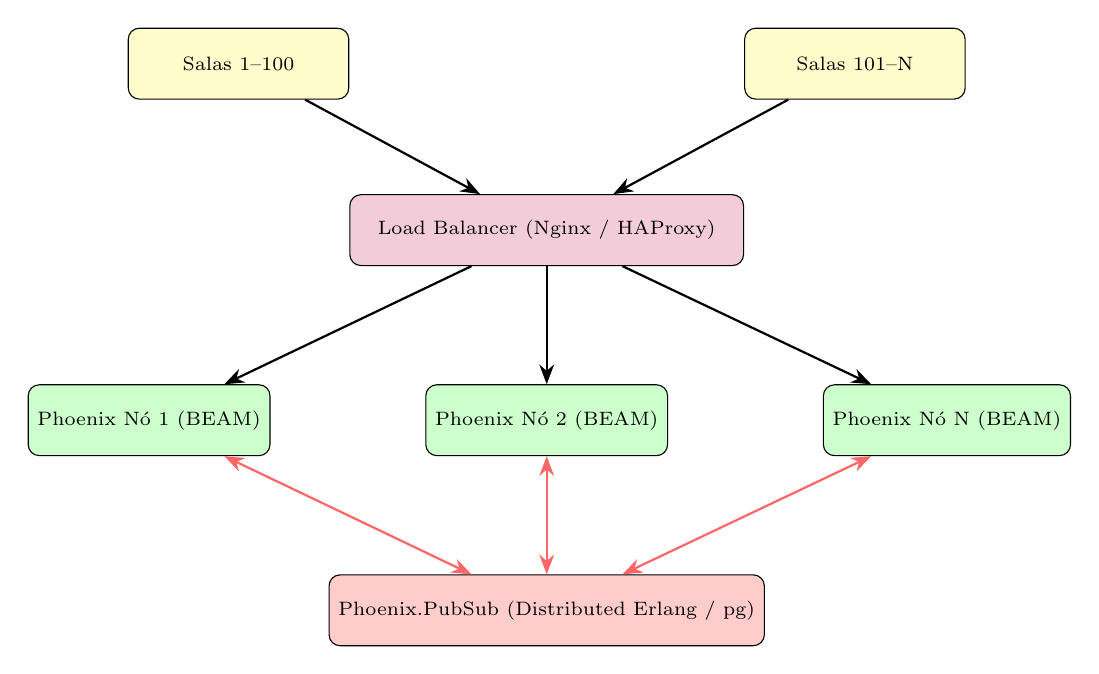
\begin{tikzpicture}[
  node distance=1.2cm,
  box/.style={rectangle, draw, rounded corners, minimum width=2.8cm, minimum height=0.9cm, text centered, font=\scriptsize},
  arrow/.style={-{Stealth[length=2.5mm]}, thick},
  doublearrow/.style={{Stealth[length=2.5mm]}-{Stealth[length=2.5mm]}, thick},
]

% Load Balancer
\node[box, fill=purple!20, minimum width=5cm] (lb) {Load Balancer (Nginx / HAProxy)};

% Instâncias Phoenix/Elixir
\node[box, fill=green!20, below left=1.5cm and 1cm of lb] (inst1) {Phoenix Nó 1 (BEAM)};
\node[box, fill=green!20, below=1.5cm of lb] (inst2) {Phoenix Nó 2 (BEAM)};
\node[box, fill=green!20, below right=1.5cm and 1cm of lb] (inst3) {Phoenix Nó N (BEAM)};

% PubSub
\node[box, fill=red!20, below=1.5cm of inst2, minimum width=5cm] (redis) {Phoenix.PubSub (Distributed Erlang / pg)};

% Setas
\draw[arrow] (lb) -- (inst1);
\draw[arrow] (lb) -- (inst2);
\draw[arrow] (lb) -- (inst3);
\draw[doublearrow, red!60] (inst1) -- (redis);
\draw[doublearrow, red!60] (inst2) -- (redis);
\draw[doublearrow, red!60] (inst3) -- (redis);

% Clientes
\node[box, fill=yellow!20, above left=1.2cm and 0cm of lb] (clients1) {Salas 1--100};
\node[box, fill=yellow!20, above right=1.2cm and 0cm of lb] (clients2) {Salas 101--N};
\draw[arrow] (clients1) -- (lb);
\draw[arrow] (clients2) -- (lb);

\end{tikzpicture}
\end{center}
\legend{Fonte: Elaborado pelo autor.}
\end{figure}

\subsubsection{Análise Comparativa de Capacidade}

A \autoref{tab:escalabilidade} compara as estratégias de escalabilidade disponíveis para a plataforma ExoGame.

\begin{table}[htb]
\caption{\label{tab:escalabilidade}Comparativo de estratégias de escalabilidade do backend Phoenix/Elixir}
\begin{tabular}{p{3cm}|p{3cm}|p{3cm}|p{3.5cm}}
  \toprule
  \textbf{Estratégia} & \textbf{Salas simultâneas} & \textbf{Jogadores estimados} & \textbf{Complexidade de implantação} \\
  \midrule
  Nó único BEAM & $\sim$2.000--10.000 & $\sim$20.000--100.000 & Mínima \\
  \midrule
  Cluster Erlang (3 nós) & $\sim$30.000+ & $\sim$300.000+ & Baixa \\
  \midrule
  Cluster + Ecto/PostgreSQL & $\sim$100.000+ & $\sim$1.000.000+ & Moderada \\
  \midrule
  Kubernetes + libcluster + CDN & Ilimitado\textsuperscript{*} & Ilimitado\textsuperscript{*} & Alta \\
  \bottomrule
\end{tabular}
\legend{Fonte: Elaborado pelo autor. \textsuperscript{*}Limitado por recursos de infraestrutura.}
\end{table}

É importante destacar que a versão atual do ExoGame utiliza o \textit{backend} Phoenix/Elixir com armazenamento em memória no \texttt{GameServer} (GenServer), adequado para o contexto acadêmico. A escalabilidade horizontal é facilitada pelo modelo de atores do Elixir/OTP, que permite adicionar nós ao \textit{cluster} sem alterar o código --- demonstrando o princípio de \textbf{transparência de localização} (\textit{location transparency}) \cite{armstrong2013}.

\subsection{WhatsApp e a BEAM: A Prova Industrial da Superioridade Erlang para WebSocket}\label{sec:whatsapp}

A escolha do Phoenix/Elixir como \textit{backend} do ExoGame não é um experimento acadêmico isolado: ela é referendada por um dos casos de escalabilidade mais citados da história da engenharia de \textit{software}. O \textbf{WhatsApp}, fundado em 2009 por Jan Koum e Brian Acton, adotou o \textbf{Erlang} (a linguagem que originou a BEAM, sobre a qual o Elixir é executado) como pilar tecnológico central de sua infraestrutura de mensagens.

\subsubsection{A Migração do WhatsApp para Erlang/BEAM}

A razão para a escolha do Erlang foi objetiva: nenhuma outra tecnologia disponível em 2009 oferecia, de forma nativa, as três propriedades simultaneamente necessárias para um sistema de mensagens global:

\begin{enumerate}
  \item \textbf{Conexões WebSocket/TCP persistentes em escala}: o modelo de ator da BEAM aloca um processo Erlang leve ($\sim$300 bytes de memória mínima) por conexão, sem âncoras no sistema operacional como \textit{threads} ou \textit{file descriptors} excessivos;
  \item \textbf{Tolerância a falhas nativa via OTP}: a árvore de supervisores OTP reinicia processos falhos automaticamente, garantindo alta disponibilidade sem intervenção manual;
  \item \textbf{Latência estável e previsível}: o \textit{scheduler} preemptivo da BEAM distribui o tempo de CPU entre todos os processos de forma equitativa, evitando que um processo monopolize o processador e cause latência imprevista.
\end{enumerate}

\subsubsection{Marcos de Escalabilidade do WhatsApp com BEAM}

Os resultados publicados pela equipe de engenharia do WhatsApp são notáveis:

\begin{itemize}
  \item Em \textbf{2011}, Rick Reed (WhatsApp) relatou \textbf{1 milhão de conexões TCP simultâneas} em um único servidor FreeBSD executando Erlang, quebrando a barreira do ``C10k problem'' por um fator de 100;
  \item Em \textbf{2012}, a equipe publicou que havia alcançado \textbf{2 milhões de conexões simultâneas por servidor}, com consumo de memória de apenas $\sim$1 GB para todo o conjunto de conexões;
  \item Em \textbf{2014}, pa poucos dias após a aquisição pelo Facebook por US\$ 19 bilhões, o WhatsApp tinha \textbf{450 milhões de usuários ativos mensais} gerenciados por uma equipe de apenas 32 engenheiros de \textit{software} --- rázio de eficiência possível em grande parte pela confiabilidade e pela baixa demanda operacional da BEAM;
  \item A arquitetura Erlang permitiu que o WhatsApp operasse com uma \textbf{frota de servidores ordens de magnitude menor} do que seria necessário com tecnologias baseadas em \textit{threads} (Java, C++) ou \textit{event loop} (Node.js), resultando em economia substancial de infraestrutura.
\end{itemize}

\subsubsection{Paralelismo com o ExoGame}

Embora a escala do ExoGame seja ordens de magnitude menor que a do WhatsApp, o \textbf{problema fundamental é arquiteturalmente idêntico}: ambos os sistemas demandam \textbf{múltiplas conexões WebSocket persistentes e simultâneas}, com eventos sendo transmitidos para grupos (\textit{rooms} no ExoGame; grupos de bate-papo no WhatsApp) em tempo real.

O Phoenix Channels do ExoGame opera exatamente sobre o mesmo modelo de atores que o Erlang do WhatsApp:

\begin{itemize}
  \item Cada conexão WebSocket é um processo Erlang isolado, supervisionado;
  \item O \texttt{Phoenix.PubSub} distribui eventos (``nova pergunta'', ``leaderboard atualizado'') entre todos os processos de uma sala de forma eficiente;
  \item Uma falha em uma sala não afeta outras salas --- isolamento garantido pela árvore de supervisores OTP.
\end{itemize}

Os resultados empíricos confirmam essa analogia: o \textit{backend} Phoenix do ExoGame sustentou \textbf{200 conexões WebSocket simultâneas com zero erros} (\autoref{sec:desempenho}). Em hardware de produção, o Phoenix poderia facilmente atingir dezenas de milhares de conexões simultâneas --- a mesma escala que tornou o WhatsApp viável com uma equipe pequena.

O modelo de concorrência do Erlang, herdado integralmente pelo Elixir, é concorrente \textbf{por padrão e não por acidente}: cada processo é isolado, leve e supervisionado, e essa propriedade estrutural é o que permite que sistemas tão distintos em escala --- o WhatsApp e o ExoGame --- compartilhem a mesma base arquitetural com o mesmo grau de confiabilidade \cite{armstrong2013}.

\subsection{Comparativo de Tecnologias}

A \autoref{tab:comparativo} apresenta um comparativo entre as tecnologias empregadas no \textit{frontend} e no \textit{backend} da plataforma ExoGame.

\begin{table}[htb]
\caption{\label{tab:comparativo}Comparativo entre as tecnologias do \textit{frontend} e \textit{backend}}
\begin{tabular}{p{3.5cm}|p{5.5cm}|p{5.5cm}}
  \toprule
  \textbf{Aspecto} & \textbf{Frontend (Next.js 15)} & \textbf{Backend (Phoenix 1.7 / Elixir)} \\
  \midrule
  Linguagem & TypeScript (React 19) & Elixir (BEAM/OTP) \\
  \midrule
  Paradigma & Componentes funcionais com Hooks & Modelo de Atores + Processos OTP (funcional) \\
  \midrule
  Renderização & SSR / ISR / Turbopack & --- \\
  \midrule
  Estilização & Tailwind CSS 4 & --- \\
  \midrule
  WebSocket & phoenix.js (Phoenix Channels client) & Phoenix Channels (RFC 6455 nativo) \\
  \midrule
  Gerenciamento de estado & Context API + useState & \texttt{GameServer} (GenServer) em memória \\
  \midrule
  Validação & Validação em formulários & \textit{Pattern matching} nativo + guardas Elixir \\
  \midrule
  Arquitetura & App Router + Componentes & Canais + GenServer + Supervisores OTP \\
  \bottomrule
\end{tabular}
\legend{Fonte: Elaborado pelo autor.}
\end{table}

\section{Ensino de Astronomia e Divulgação Científica}\label{sec:astronomia}

\subsection{Situação do Ensino de Astronomia no Brasil}

\citeonline{langhi2009} realizaram uma extensa revisão sobre o ensino de Astronomia no Brasil, identificando deficiências tanto na formação de professores quanto na disponibilidade de recursos didáticos adequados. Os autores apontam que, embora a Astronomia desperte grande interesse e curiosidade nos estudantes, sua abordagem em sala de aula frequentemente se limita a descrições superficiais do Sistema Solar.

A escassez de ferramentas interativas e contextualizadas para o ensino de conceitos astronômicos mais avançados --- como a detecção e caracterização de exoplanetas --- constitui uma barreira significativa para a alfabetização científica nessa área.

\subsection{Exoplanetas: Uma Trajetória Histórica de Quatro Séculos}

A ideia de que outros mundos possam existir além do Sistema Solar não é uma concepção moderna. Ao contrário, trata-se de uma das mais antigas e persistentes questões da história do pensamento humano, cuja trajetória intelectual percorre quatro séculos de especulação filosófica, fundamentação teórica e, finalmente, confirmação observacional. Esta subseção reconstrói essa trajetória de modo didático, desde os primeiros visionários até as missões espaciais contemporâneas.

\subsubsection{Os Precursores Filosóficos: De Epicuro a Giordano Bruno}

A noção de pluralidade de mundos encontra raízes na filosofia grega antiga. \textbf{Epicuro} (341--270 a.C.), seguindo o atomismo de Demócrito, argumentava que, se o número de átomos é infinito e o espaço também, então é inevitável que existam outros mundos semelhantes ao nosso. Em sua \textit{Carta a Heródoto}, Epicuro afirmou: ``existem infinitos mundos, alguns semelhantes a este e outros diferentes'' \cite{dick1982}.

Contudo, foi o filósofo e frei dominicano italiano \textbf{Giordano Bruno} (1548--1600) quem articulou de forma mais radical e influente a tese da pluralidade dos mundos na era moderna. Em sua obra \textit{De l'Infinito, Universo e Mondi} (``Sobre o Infinito, o Universo e os Mundos''), publicada em 1584, Bruno propôs que:

\begin{itemize}
  \item O universo é \textbf{infinito} e não possui centro;
  \item As estrelas são \textbf{sóis distantes}, cada uma potencialmente cercada por seus próprios planetas;
  \item Esses planetas podem abrigar \textbf{formas de vida}, assim como a Terra \cite{bruno1584}.
\end{itemize}

Bruno rejeitava explicitamente o modelo geocêntrico e mesmo o heliocentrismo limitado de Copérnico --- para Bruno, o Sol não era o centro do universo, mas apenas mais uma estrela entre infinitas. Essa visão cosmológica, somada às suas posições teológicas heterodoxas, levou-o à condenação pela Inquisição e à execução na fogueira em 1600. Embora Bruno não dispusesse de qualquer meio observacional para verificar suas hipóteses, sua intuição sobre a existência de planetas extrasolares mostrou-se extraordinariamente presciente à luz das descobertas modernas.

\subsubsection{O Período Newtoniano e os Primeiros Cálculos}

A revolução científica dos séculos XVII e XVIII forneceu os alicerces teóricos para transformar a questão dos exoplanetas de especulação filosófica em problema científico. \textbf{Isaac Newton} (1643--1727), ao formular a lei da gravitação universal na \textit{Principia Mathematica} (1687), demonstrou que as mesmas leis físicas que governam o Sistema Solar aplicam-se a todo o universo observável \cite{newton1687}. Essa universalidade da gravidade implicava que estrelas distantes poderiam, em princípio, manter sistemas planetários gravitacionalmente ligados.

\textbf{Christiaan Huygens} (1629--1695), em sua obra póstuma \textit{Cosmotheoros} (1698), foi além ao calcular semelhanças entre o Sol e as estrelas com base em suas luminosidades. Huygens argumentou que, se as estrelas são sóis, seria razoável supor que também possuem planetas \cite{huygens1698}. Ele tentou inclusive estimar o tamanho e a distância das estrelas comparando seu brilho com o do Sol --- método rudimentar, mas conceitualmente precursor da fotometria estelar.

\subsubsection{Século XIX: Primeiras Tentativas de Detecção}

O século XIX trouxe as primeiras tentativas concretas de detecção de exoplanetas por meio da \textbf{astrometria} --- a medição precisa das posições das estrelas no céu. O princípio é elegante: se um planeta orbita uma estrela, a atração gravitacional mútua faz com que a estrela ``oscile'' em torno do centro de massa do sistema, produzindo um deslocamento minúsculo em sua posição aparente.

Em 1855, o capitão \textbf{William Stephen Jacob}, do observatório de Madras (Índia), reportou anomalias na órbita do sistema binário 70 Ophiuchi que poderiam ser explicadas pela presença de um corpo planetário \cite{jacob1855}. Essa alegação foi posteriormente refutada, mas inaugurou uma longa tradição de tentativas astrométricas.

No início do século XX, \textbf{Peter van de Kamp} (1901--1995), astrônomo holandês-americano do Observatório Sproul, dedicou décadas à busca de perturbações astrométricas na \textbf{Estrela de Barnard}. Entre 1963 e 1969, Van de Kamp publicou artigos afirmando ter detectado um ou dois companheiros planetários \cite{vandekamp1963}. Essas descobertas atraíram enorme atenção, mas foram progressivamente contestadas quando se demonstrou que as perturbações eram artefatos instrumentais causados por ajustes nas lentes do telescópio \cite{gatewood1973}. O episódio de Van de Kamp, embora frustrante, foi educativo: estabeleceu a necessidade de rigor instrumental extremo e controle de erros sistemáticos na busca por exoplanetas.

\subsubsection{A Proposta de Otto Struve e os Métodos Indiretos}

O astrônomo russo-americano \textbf{Otto Struve} (1897--1963) publicou em 1952 um artigo visionário no qual propôs dois métodos que se tornariam os pilares da detecção de exoplanetas décadas mais tarde \cite{struve1952}:

\begin{enumerate}
  \item \textbf{Velocidade radial} (ou efeito Doppler espectroscópico): se um planeta orbita uma estrela, a estrela se move periodicamente em relação ao observador, causando deslocamentos mensuráveis nas linhas espectrais. Struve estimou que um planeta do tamanho de Júpiter em órbita próxima à estrela produziria variações de velocidade radial de dezenas de metros por segundo --- valores que, embora desafiadores, estavam dentro do alcance conceitual de espectrógrafos de alta resolução;

  \item \textbf{Trânsito fotométrico}: se a órbita de um planeta estiver alinhada com a linha de visada do observador, o planeta cruzará periodicamente o disco estelar, causando uma diminuição minúscula no brilho observado. Struve estimou que um Júpiter quente poderia causar uma queda de $\sim$1\% na luminosidade estelar.
\end{enumerate}

A previsão de Struve sobre a existência de ``Júpiteres quentes'' --- planetas gigantes em órbitas muito próximas --- antecipou em mais de 40 anos a descoberta de 51 Pegasi b, demonstrando notável insight astrofísico.

\subsubsection{A Primeira Detecção: Planetas ao Redor de um Pulsar (1992)}

Paradoxalmente, os primeiros exoplanetas confirmados não foram encontrados ao redor de uma estrela convencional, mas sim de um \textbf{pulsar} --- uma estrela de nêutrons remanescente de uma explosão de supernova. Em 1992, os astrônomos \textbf{Aleksander Wolszczan} e \textbf{Dale Frail} publicaram na revista \textit{Nature} a detecção de dois planetas orbitando o pulsar PSR B1257+12, utilizando o método de cronometragem de pulsos \cite{wolszczan1992}.

Os pulsares emitem pulsos de rádio com regularidade extraordinária --- comparável a relógios atômicos. Se um ou mais planetas orbitam o pulsar, as variações gravitacionais induzem atrasos e adiantamentos periódicos nos tempos de chegada dos pulsos, com precisão de nanosegundos. Wolszczan e Frail detectaram dois planetas com massas de aproximadamente 4,3 e 3,9 vezes a massa da Terra, com períodos orbitais de 66,5 e 98,2 dias, respectivamente.

Essa descoberta, embora historicamente monumental, não gerou o entusiasmo público esperado. Planetas ao redor de pulsares são formados em condições extremas (possivelmente a partir de material reacumulado após a supernova) e são inóspitos por definição. A comunidade científica ansiava pela detecção de planetas ao redor de estrelas ``normais'' --- de sequência principal, semelhantes ao Sol.

\subsubsection{A Revolução de 1995: 51 Pegasi b e o Júpiter Quente}

A descoberta que transformou o campo ocorreu em outubro de 1995, quando \textbf{Michel Mayor} e \textbf{Didier Queloz}, do Observatório de Genebra, anunciaram a detecção de um planeta orbitando a estrela 51 Pegasi, uma estrela de tipo solar na constelação de Pegasus \cite{mayor1995}. Utilizando o espectrógrafo ELODIE instalado no Observatório de Haute-Provence, na França, Mayor e Queloz mediram variações periódicas de velocidade radial de $\sim$59 m/s com período de apenas 4,23 dias.

Os parâmetros de 51 Pegasi b surpreenderam a comunidade: um planeta com massa mínima de 0,47 $M_J$ (massas de Júpiter) orbitando a apenas 0,052 UA da estrela --- muito mais próximo do que Mercúrio está do Sol. Nenhum modelo de formação planetária vigente na época previa a existência de gigantes gasosos tão próximos de suas estrelas hospedeiras. Esses objetos, batizados de \textbf{``Júpiteres quentes''} (\textit{hot Jupiters}), exigiram uma revisão profunda das teorias de formação e migração planetária \cite{perryman2018}.

A descoberta rendeu a Mayor e Queloz o \textbf{Prêmio Nobel de Física de 2019}, compartilhado com James Peebles (por contribuições à cosmologia teórica), consolidando o estudo de exoplanetas como um dos campos mais relevantes da astrofísica contemporânea.

\subsubsection{A Era Kepler: A Explosão Estatística (2009--2018)}

A missão \textit{Kepler} da NASA, lançada em março de 2009, representou um salto quantitativo sem precedentes na detecção de exoplanetas \cite{borucki2010}. Equipado com um fotômetro de altíssima precisão, o \textit{Kepler} monitorou continuamente o brilho de mais de 150.000 estrelas numa região fixa do céu (nas constelações de Cygnus e Lyra) durante quatro anos, buscando as diminuições periódicas causadas pelo trânsito de planetas.

Os resultados foram revolucionários:

\begin{itemize}
  \item Mais de \textbf{2.700 exoplanetas confirmados} diretamente pela missão;
  \item A demonstração de que \textbf{planetas rochosos do tamanho da Terra são comuns} na galáxia --- uma conclusão estatística de enorme implicação para a questão da vida extraterrestre;
  \item A descoberta de \textbf{arquiteturas planetárias diversas}: sistemas com múltiplos planetas em ressonância orbital, planetas circumbinários (orbitando duas estrelas), planetas em órbitas extremamente excêntricas;
  \item A identificação de planetas na \textbf{zona habitável} de suas estrelas, como o Kepler-22b (primeiro planeta confirmado na zona habitável de uma estrela semelhante ao Sol) e os planetas do sistema Kepler-186 (primeiro planeta do tamanho da Terra em zona habitável) \cite{nasaexoplanet2024};
  \item O resultado estatístico mais impactante: extrapolando os dados do \textit{Kepler}, estimou-se que existam \textbf{mais planetas do que estrelas na Via Láctea} --- pelo menos 100 bilhões de planetas apenas em nossa galáxia.
\end{itemize}

A missão estendida \textit{K2} (2014--2018), conduzida após a falha de duas das quatro rodas de reação do satélite, continuou a produzir resultados científicos significativos, observando campos estelares diferentes ao longo da eclíptica.

\subsubsection{TESS e a Era Atual (2018--Presente)}

O \textit{Transiting Exoplanet Survey Satellite} (\textbf{TESS}), lançado em abril de 2018, foi projetado como o sucessor natural do \textit{Kepler} \cite{ricker2015}. Enquanto o \textit{Kepler} observou uma região fixa e profunda do céu, o TESS realiza um \textbf{levantamento quase completo do céu}, monitorando as 200.000 estrelas mais brilhantes e próximas. Essa estratégia é complementar: o TESS identifica planetas ao redor de estrelas brilhantes que são ideais para caracterização atmosférica por telescópios como o \textit{James Webb Space Telescope} (JWST).

Desde seu lançamento, o TESS já identificou mais de 7.000 candidatos a exoplanetas (TOIs --- \textit{TESS Objects of Interest}), dos quais centenas já foram confirmados, incluindo mundos rochosos em zonas habitáveis de estrelas anãs vermelhas \cite{nasaexoplanet2024}.

O \textbf{JWST}, lançado em dezembro de 2021, inaugurou uma nova era ao permitir a \textbf{espectroscopia de atmosferas} de exoplanetas com resolução sem precedentes. Em 2022, o JWST detectou dióxido de carbono (CO$_2$) na atmosfera do exoplaneta WASP-39b --- a primeira detecção inequívoca de uma molécula específica na atmosfera de um exoplaneta por observação direta \cite{jwst2023}. Essa capacidade abre caminho para a busca por \textbf{biomarcadores} --- moléculas como oxigênio, metano e vapor d'água cuja presença simultânea poderia indicar atividade biológica.

\subsubsection{Linha do Tempo: Marcos na História dos Exoplanetas}

A \autoref{tab:timeline_exoplanetas} sintetiza os marcos fundamentais na trajetória de quatro séculos de busca por mundos extrasolares.

\begin{table}[htb]
\caption{\label{tab:timeline_exoplanetas}Linha do tempo dos marcos na história dos exoplanetas}
\begin{tabular}{p{1.5cm}|p{3.5cm}|p{8.5cm}}
  \toprule
  \textbf{Ano} & \textbf{Protagonista(s)} & \textbf{Contribuição} \\
  \midrule
  1584 & Giordano Bruno & Propõe estrelas como sóis com planetas próprios (\textit{De l'Infinito}) \\
  \midrule
  1698 & Christiaan Huygens & Argumenta pela pluralidade de mundos em \textit{Cosmotheoros} \\
  \midrule
  1952 & Otto Struve & Propõe detecção por velocidade radial e trânsito fotométrico \\
  \midrule
  1963 & Peter van de Kamp & Alega (erroneamente) planetas na Estrela de Barnard \\
  \midrule
  1992 & Wolszczan \& Frail & Primeiros exoplanetas confirmados (pulsar PSR B1257+12) \\
  \midrule
  1995 & Mayor \& Queloz & 51 Pegasi b --- primeiro exoplaneta em estrela tipo solar \\
  \midrule
  1999 & Charbonneau et al. & Primeiro trânsito de exoplaneta observado (HD 209458 b) \\
  \midrule
  2009 & Missão \textit{Kepler} & Lançamento; detectará mais de 2.700 exoplanetas \\
  \midrule
  2014 & Kepler-186f & Primeiro planeta do tamanho da Terra em zona habitável \\
  \midrule
  2017 & TRAPPIST-1 & Sistema com 7 planetas rochosos, 3 em zona habitável \\
  \midrule
  2018 & TESS & Levantamento do céu inteiro; milhares de candidatos \\
  \midrule
  2022 & JWST & Primeira detecção de CO$_2$ em atmosfera exoplanetária \\
  \midrule
  2024 & Catálogo NASA & Mais de 5.700 exoplanetas confirmados \\
  \bottomrule
\end{tabular}
\legend{Fonte: Elaborado pelo autor com base em \citeonline{perryman2018} e \citeonline{nasaexoplanet2024}.}
\end{table}

\subsubsection{Significado para a Educação Científica}

A trajetória histórica dos exoplanetas possui imenso potencial pedagógico. Ela ilustra conceitos fundamentais da epistemologia científica: a longa gestação de uma ideia desde a especulação filosófica até a confirmação observacional; a importância da tecnologia instrumental na validação de hipóteses; o papel do erro e da refutação (caso Van de Kamp) no progresso científico; e a natureza acumulativa do conhecimento, na qual cada geração constrói sobre os ombros da anterior.

Ao integrar essa narrativa histórica nas questões do ExoGame, a plataforma transcende a mera verificação de fatos pontuais e convida o estudante a compreender a ciência como \textbf{processo} --- uma lição que, segundo \citeonline{langhi2009}, é frequentemente negligenciada no ensino convencional de Astronomia. A diversidade de exoplanetas descobertos --- \textit{super-Terras}, \textit{mini-Netunos}, planetas em zona habitável, sistemas multiplanetários --- oferece um vasto campo para atividades didáticas que podem despertar a curiosidade científica e promover o letramento astronômico.

\subsection{Acurácia Científica: O NASA Exoplanet Archive como Fonte Primária}\label{sec:acuracia}

Um diferencial fundamental de qualquer ferramenta de divulgação científica é a \textbf{acurácia dos dados} apresentados. No contexto de plataformas gamificadas, onde o engajamento lúdico pode, inadvertidamente, comprometer o rigor informacional, a ancoragem em fontes primárias revisadas por pares torna-se uma exigência epistemológica. O ExoGame endereça essa preocupação ao fundamentar seu banco de questões no \textbf{NASA Exoplanet Archive} \cite{nasaexoplanet2024, akeson2013}.

\subsubsection{Caracterização do NASA Exoplanet Archive}

O NASA Exoplanet Archive, mantido pelo \textit{NASA Exoplanet Science Institute} (NExScI) no \textit{California Institute of Technology} (Caltech), é o repositório oficial de dados sobre exoplanetas confirmados e candidatos \cite{akeson2013}. Suas características incluem:

\begin{itemize}
  \item \textbf{Cobertura}: dados de mais de 5.700 exoplanetas confirmados (até 2025), incluindo parâmetros orbitais, estelares e atmosféricos;
  \item \textbf{Curadoria científica}: cada entrada passa por processo de revisão que verifica a publicação em periódicos indexados e a consistência dos parâmetros reportados;
  \item \textbf{Atualização contínua}: novos planetas são incorporados à medida que publicações são aceitas, mantendo o catálogo atualizado com as descobertas mais recentes;
  \item \textbf{API pública}: oferece acesso programático via TAP (\textit{Table Access Protocol}) e CSV, permitindo a integração automatizada com sistemas externos;
  \item \textbf{Dados compostos}: agrega resultados de múltiplas missões (\textit{Kepler}, \textit{TESS}, observações de velocidade radial, imageamento direto), oferecendo uma visão consolidada do conhecimento atual.
\end{itemize}

\subsubsection{Protocolo de Elaboração de Questões}

O banco de questões do ExoGame segue um protocolo de elaboração que garante validade científica:

\begin{enumerate}
  \item \textbf{Consulta à fonte primária}: cada questão sobre exoplanetas específicos é verificada contra os dados do NASA Exoplanet Archive, assegurando que parâmetros como raio, período orbital, método de detecção e classificação estejam corretos;
  \item \textbf{Contextualização pedagógica}: o campo \texttt{correctAnswerContext} da interface \texttt{Question} fornece uma explicação didática que conecta o dado científico ao contexto mais amplo do conhecimento astronômico;
  \item \textbf{Rastreabilidade}: as questões podem ser associadas a referências bibliográficas específicas (artigos de descoberta, catálogos de missões), permitindo que professores e alunos acessem as fontes originais;
  \item \textbf{Validação cruzada}: dados sobre exoplanetas são cruzados com publicações em periódicos como \textit{The Astrophysical Journal}, \textit{Astronomy \& Astrophysics} e \textit{Nature}, que são as fontes primárias do próprio Archive.
\end{enumerate}

\subsubsection{Validade Científica como Diferencial Pedagógico}

A ancoragem em dados reais do NASA Exoplanet Archive confere ao ExoGame um diferencial crítico em relação a quizzes genéricos: a \textbf{validade científica}. Segundo \citeonline{langhi2009}, um dos problemas recorrentes no ensino de Astronomia é a presença de concepções alternativas (``misconceptions'') perpetuadas por materiais didáticos desatualizados ou imprecisos. Ao utilizar o catálogo oficial da NASA como fonte, o ExoGame mitiga esse risco e contribui para a formação de uma base conceitual cientificamente acurada.

Além disso, essa abordagem alinha-se com a perspectiva de \citeonline{ausubel2000} sobre a importância da \textit{validade substantiva} do material de aprendizagem: para que ocorra aprendizagem significativa, o conteúdo não pode ser trivial ou fictício --- ele deve possuir significado lógico legítimo. Ao basear-se em descobertas reais de exoplanetas, o ExoGame satisfaz essa condição, pois cada pergunta reflete um fato científico verificável.

A \autoref{tab:exemplos_questoes} exemplifica como os dados do NASA Exoplanet Archive são transpostos para questões do ExoGame.

\begin{table}[htb]
\caption{\label{tab:exemplos_questoes}Exemplos de transposição de dados NASA para questões do ExoGame}
\begin{tabular}{p{2.5cm}|p{3.5cm}|p{4cm}|p{3.5cm}}
  \toprule
  \textbf{Dado NASA} & \textbf{Parâmetro} & \textbf{Questão gerada} & \textbf{Contexto educativo} \\
  \midrule
  Kepler-22b & Zona habitável confirmada & ``Qual exoplaneta foi o primeiro confirmado em zona habitável pela missão Kepler?'' & Conceito de zona habitável e método de trânsito \\
  \midrule
  TRAPPIST-1 & 7 planetas rochosos & ``Quantos planetas foram descobertos no sistema TRAPPIST-1?'' & Sistemas multiplanetários e estrelas anãs \\
  \midrule
  51 Pegasi b & Primeiro exoplaneta em estrela solar & ``Qual foi o primeiro exoplaneta descoberto orbitando uma estrela tipo solar?'' & História da detecção e velocidade radial \\
  \midrule
  HD 209458 b & Primeiro trânsito observado & ``Qual exoplaneta teve o primeiro trânsito atmosférico detectado?'' & Espectroscopia de trânsito \\
  \bottomrule
\end{tabular}
\legend{Fonte: Elaborado pelo autor com dados do NASA Exoplanet Archive \cite{nasaexoplanet2024}.}
\end{table}

\subsubsection{Banco de Questões Implementado}\label{sec:banco_questoes}

O ExoGame disponibiliza 20 questões científicas sobre exoplanetas, todas fundamentadas em dados primários do NASA Exoplanet Archive \cite{nasaexoplanet2024, akeson2013} e em publicações revisadas por pares. Estas questões foram implementadas no módulo \texttt{QuestionService} do \textit{backend} Phoenix/Elixir e validadas experimentalmente via testes de integração (resposta HTTP~200, 20 questões retornadas, estrutura de campos verificada).

O \autoref{quad:banco_questoes} apresenta o banco completo com a resposta correta, o tema abordado e a referência bibliográfica de cada questão.

\begin{quadro}[htb]
\caption{\label{quad:banco_questoes}Banco de questões sobre exoplanetas implementado no ExoGame}
\begin{tabular}{|p{0.4cm}|p{6.3cm}|p{3.0cm}|p{1.8cm}|p{2.2cm}|}
  \hline
  \textbf{\#} & \textbf{Questão} & \textbf{Resposta correta} & \textbf{Tema} & \textbf{Referência} \\ \hline
  1 & Qual foi o primeiro exoplaneta confirmado orbitando uma estrela tipo solar, descoberto em 1995? & 51 Pegasi b & História & \citeonline{mayor1995} \\ \hline
  2 & Qual método detecta exoplanetas medindo a queda periódica no brilho de uma estrela? & Método de Trânsito & Métodos & \citeonline{borucki2010} \\ \hline
  3 & Quantos planetas rochosos foram descobertos no sistema TRAPPIST-1? & 7 & Sistemas & \citeonline{gillon2017} \\ \hline
  4 & Qual missão da NASA descobriu mais de 2.600 exoplanetas entre 2009 e 2018? & Kepler & Missões & \citeonline{borucki2010} \\ \hline
  5 & Em 1992, ao redor de que tipo de objeto foram descobertos os primeiros exoplanetas? & Pulsar & História & \citeonline{wolszczan1992} \\ \hline
  6 & Qual foi o primeiro exoplaneta a ter sua atmosfera detectada (H, He, C)? & HD~209458b & Atmosferas & \citeonline{vidalmadjur2003} \\ \hline
  7 & Qual é o exoplaneta mais próximo do Sol, em zona habitável da anã vermelha? & Proxima Centauri b & Vizinhança & \citeonline{anglada2016} \\ \hline
  8 & O método de velocidade radial detecta exoplanetas medindo qual fenômeno? & O efeito Doppler & Métodos & \citeonline{mayor1995} \\ \hline
  9 & Qual telescópio, lançado em 2021, fez a 1\textsuperscript{a} detecção de CO\textsubscript{2} em exoplaneta? & James Webb (JWST) & Missões & \citeonline{gardner2006} \\ \hline
  10 & Quantos exoplanetas confirmados existiam no NASA Exoplanet Archive até 2025? & Mais de 5.700 & Catálogos & \citeonline{nasaexoplanet2024} \\ \hline
  \multicolumn{5}{r|}{\footnotesize\textit{continua\ldots}} \\ \hline
\end{tabular}
\end{quadro}

\addtocounter{quadro}{-1}
\begin{quadro}[htb]
\caption{(continuação) Banco de questões sobre exoplanetas implementado no ExoGame}
\begin{tabular}{|p{0.4cm}|p{6.3cm}|p{3.0cm}|p{1.8cm}|p{2.2cm}|}
  \hline
  \textbf{\#} & \textbf{Questão} & \textbf{Resposta correta} & \textbf{Tema} & \textbf{Referência} \\ \hline
  11 & Como se chama o fenômeno em que a gravidade curva a luz de uma estrela de fundo? & Microlente Gravitacional & Métodos & \citeonline{perryman2018} \\ \hline
  12 & Os ``Júpiteres quentes'' têm qual característica orbital marcante? & Período orbital curto (dias) & Tipos & \citeonline{mayor1995} \\ \hline
  13 & Qual missão da NASA, lançada em 2018, monitora estrelas brilhantes próximas? & TESS & Missões & \citeonline{ricker2015} \\ \hline
  14 & O sistema TRAPPIST-1 está a aproximadamente quantos anos-luz da Terra? & 40 & Sistemas & \citeonline{gillon2017} \\ \hline
  15 & O que define a ``zona habitável'' (\textit{Zona de Goldilocks}) de uma estrela? & Permite água líquida na superfície & Habitabilidade & \citeonline{kasting1993} \\ \hline
  16 & Qual o período orbital aproximado de Kepler-452b, o ``primo da Terra''? & $\approx$385 dias & Sistemas & \citeonline{jenkins2015} \\ \hline
  17 & O imageamento direto é mais eficaz para detectar qual tipo de exoplaneta? & Gigantes jovens e distantes & Métodos & \citeonline{perryman2018} \\ \hline
  18 & Quem propôs em 1952 que planetas poderiam ser detectados por variações espectrais? & Otto Struve & História & \citeonline{struve1952} \\ \hline
  19 & Qual missão europeia (2019) mede raios de exoplanetas para calcular densidades? & CHEOPS & Missões & \citeonline{benz2021} \\ \hline
  20 & O JWST detectou em 2023 sinais de DMS em qual exoplaneta? & K2-18b & Atmosferas & \citeonline{madhusudhan2023} \\ \hline
\end{tabular}
\fonte{Elaborado pelo autor. Questões implementadas em \texttt{backend/src/question/question.service.ts}, validadas por teste de integração (\texttt{test\_questions.mjs}). Referências: \citeonline{mayor1995, borucki2010, gillon2017, wolszczan1992, vidalmadjur2003, anglada2016, gardner2006, nasaexoplanet2024, perryman2018, ricker2015, kasting1993, jenkins2015, struve1952, benz2021, madhusudhan2023, akeson2013}.}
\end{quadro}

\subsection{Tecnologias Interativas na Divulgação Científica}

A convergência entre tecnologias \textit{web} interativas e divulgação científica tem produzido experiências educacionais transformadoras. Plataformas que permitem a manipulação de dados reais, visualizações interativas e simulações numéricas democratizam o acesso a conteúdos que antes estavam restritos ao meio acadêmico.

Nesse contexto, a proposta da plataforma ExoGame se insere como uma ponte entre a gamificação, as tecnologias \textit{web} em tempo real e a divulgação de conhecimentos sobre exoplanetas, buscando tornar acessíveis conceitos que, de outra forma, poderiam parecer abstratos e distantes da realidade dos estudantes.


% ============================================================
% CAPÍTULO 3 - METODOLOGIA
% ============================================================
\chapter{Metodologia}\label{cap:metodologia}

Este capítulo descreve a metodologia adotada para o desenvolvimento da plataforma ExoGame, incluindo a classificação da pesquisa, as ferramentas utilizadas e o processo de desenvolvimento.

\section{Classificação da Pesquisa}

Do ponto de vista dos objetivos, esta pesquisa classifica-se como \textbf{exploratória} e \textbf{aplicada}, pois visa o desenvolvimento de uma solução tecnológica concreta para um problema identificado --- a carência de ferramentas gamificadas para o ensino de Astronomia. Do ponto de vista dos procedimentos técnicos, configura-se como pesquisa bibliográfica, combinada com desenvolvimento experimental de software.

\section{Ferramentas de Desenvolvimento}

O \autoref{quad:ferramentas} apresenta as principais ferramentas e tecnologias empregadas no desenvolvimento da plataforma.

\begin{quadro}[htb]
\caption{\label{quad:ferramentas}Ferramentas e tecnologias utilizadas}
\begin{tabular}{|p{3.5cm}|p{3cm}|p{6.5cm}|}
	\hline
	\textbf{Ferramenta} & \textbf{Versão} & \textbf{Finalidade} \\ \hline
	Next.js & 15.5.2 & \textit{Framework} \textit{frontend} com SSR \\ \hline
	React & 19.1.0 & Biblioteca para construção de interfaces \\ \hline
	Elixir & 1.14+ & Linguagem funcional --- único \textit{backend} da plataforma (BEAM/OTP) \\ \hline
	Phoenix & 1.7.21 & \textit{Framework} \textit{backend} com Canais WebSocket nativos \\ \hline
	phoenix.js & 1.7.x & Biblioteca cliente Phoenix Channels (\textit{frontend}) \\ \hline
	TypeScript & 5.9.2 & Linguagem de programação tipada (\\textit{frontend}) \\ \hline
	Tailwind CSS & 4.x & \textit{Framework} de estilização utilitário \\ \hline
	Docker & 28.x & Conteinerização do \textit{backend} e \textit{frontend} \\ \hline
	Docker Compose & 2.x & Orquestração multi-contêiner com limites de CPU/RAM \\ \hline
\end{tabular}
\fonte{Elaborado pelo autor.}
\end{quadro}

\section{Processo de Desenvolvimento}

O desenvolvimento seguiu uma abordagem iterativa e incremental, organizada nas seguintes etapas:

\begin{enumerate}
  \item \textbf{Levantamento de requisitos}: definição das funcionalidades essenciais com base na análise de plataformas similares (Kahoot!, Quizizz, Socrative);
  \item \textbf{Projeto da arquitetura}: definição da arquitetura cliente-servidor, estrutura de módulos e protocolo de comunicação;
  \item \textbf{Implementação do \textit{backend}}: desenvolvimento dos canais, GenServers e serviços com Phoenix 1.7 (Elixir/BEAM);
  \item \textbf{Implementação do \textit{frontend}}: desenvolvimento da interface com Next.js e integração com o \textit{backend} via WebSocket;
  \item \textbf{Testes e validação}: testes manuais de integração com múltiplos clientes simultâneos e testes automatizados de carga (\textit{load tests}) com script Python (\ texttt{load\_test.py}), avaliando latência HTTP e conexões WebSocket sob concorrência crescente;
  \item \textbf{Conteinerização}: configuração do \texttt{docker-compose.yml} para implantação reprodutível com restrições de recursos (1 CPU, 2 GB RAM por serviço);
  \item \textbf{Documentação}: elaboração da documentação técnica e do presente trabalho acadêmico.
\end{enumerate}


% ============================================================
% CAPÍTULO 4 - ARQUITETURA DO SISTEMA
% ============================================================
\chapter{Arquitetura do Sistema}\label{cap:arquitetura}

Este capítulo detalha a arquitetura da plataforma ExoGame, incluindo a visão geral do sistema, a estrutura de módulos do \textit{backend}, a organização de componentes do \textit{frontend} e o protocolo de comunicação via WebSocket.

\section{Visão Geral da Arquitetura}

A plataforma ExoGame adota uma arquitetura \textbf{cliente-servidor} composta por dois processos independentes comunicando-se por meio de dois canais: requisições HTTP REST para consultas estáticas e WebSocket (Phoenix Channels) para interações em tempo real.

A \autoref{fig:arquitetura_geral} ilustra a visão geral da arquitetura do sistema.

\begin{figure}[htb]
\caption{\label{fig:arquitetura_geral}Arquitetura geral da plataforma ExoGame}
\begin{center}
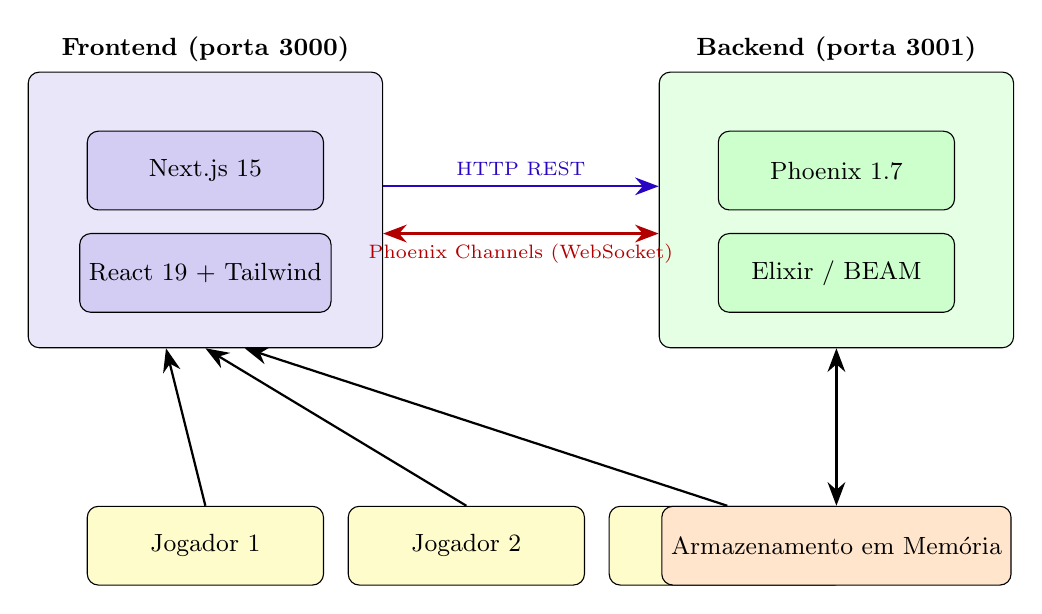
\begin{tikzpicture}[
  node distance=1.5cm,
  box/.style={rectangle, draw, rounded corners, minimum width=3cm, minimum height=1cm, text centered, font=\small},
  bigbox/.style={rectangle, draw, rounded corners, minimum width=4.5cm, minimum height=3.5cm, text centered},
  arrow/.style={-{Stealth[length=3mm]}, thick},
  doublearrow/.style={{Stealth[length=3mm]}-{Stealth[length=3mm]}, thick},
]

% Frontend
\node[bigbox, fill=blue!10, label={[font=\bfseries\small]above:Frontend (porta 3000)}] (frontend) {};
\node[box, fill=blue!20] at ([yshift=0.5cm]frontend.center) (nextjs) {Next.js 15};
\node[box, fill=blue!20] at ([yshift=-0.8cm]frontend.center) (react) {React 19 + Tailwind};

% Backend
\node[bigbox, fill=green!10, right=3.5cm of frontend, label={[font=\bfseries\small]above:Backend (porta 3001)}] (backend) {};
\node[box, fill=green!20] at ([yshift=0.5cm]backend.center) (phoenix) {Phoenix 1.7};
\node[box, fill=green!20] at ([yshift=-0.8cm]backend.center) (elixirbeam) {Elixir / BEAM};

% Setas
\draw[arrow, blue] ([yshift=0.3cm]frontend.east) -- node[above, font=\scriptsize] {HTTP REST} ([yshift=0.3cm]backend.west);
\draw[doublearrow, red!70!black] ([yshift=-0.3cm]frontend.east) -- node[below, font=\scriptsize] {Phoenix Channels (WebSocket)} ([yshift=-0.3cm]backend.west);

% Clientes
\node[box, fill=yellow!20, below=2cm of frontend] (client1) {Jogador 1};
\node[box, fill=yellow!20, right=0.3cm of client1] (client2) {Jogador 2};
\node[box, fill=yellow!20, right=0.3cm of client2] (clientn) {Jogador N};

% Setas dos clientes
\draw[arrow] (client1.north) -- ([xshift=-0.5cm]frontend.south);
\draw[arrow] (client2.north) -- (frontend.south);
\draw[arrow] (clientn.north) -- ([xshift=0.5cm]frontend.south);

% Store
\node[box, fill=orange!20, below=2cm of backend] (memory) {Armazenamento em Memória};
\draw[doublearrow] (backend.south) -- (memory.north);

\end{tikzpicture}
\end{center}
\legend{Fonte: Elaborado pelo autor.}
\end{figure}

\section{Estrutura de Módulos do \textit{Backend}}\label{sec:modulos_backend}

O \textit{backend} (Phoenix/Elixir) organiza-se em três contextos supervisionados pela árvore OTP:

\begin{enumerate}
  \item \textbf{GameChannel / GameServer}: canal principal com o \texttt{GameChannel} (Phoenix Channels via WebSocket nativo) e o \texttt{GameServer} (GenServer OTP) que mantém o estado das salas em memória;
  \item \textbf{QuestionService}: serviço de questões com dados compilados em atributo de módulo Elixir (\texttt{@questions});
  \item \textbf{PlayerService}: gerenciamento de jogadores com structs Elixir e atualização de pontuação.
\end{enumerate}

Cada contexto encapsula seus componentes (canais, serviços e processos GenServer) e expõe apenas as interfaces necessárias para outros contextos, seguindo o princípio de encapsulamento e baixo acoplamento \cite{martin2008, gamma1994}.

\section{Estrutura de Componentes do \textit{Frontend}}

O \textit{frontend} em Next.js utiliza o \textbf{App Router} e é organizado em componentes React funcionais com a seguinte hierarquia:

\begin{itemize}
  \item \textbf{RootLayout}: componente raiz que envolve toda a aplicação com o \texttt{GameProvider};
  \item \textbf{Home (page.tsx)}: página principal que renderiza condicionalmente os componentes com base no estado do jogo;
  \item \textbf{HomePage}: tela inicial com formulários para criar ou entrar em um jogo;
  \item \textbf{Lobby}: sala de espera que exibe os jogadores conectados e o código PIN;
  \item \textbf{QuestionView}: exibe a pergunta atual com temporizador, opções e barra de progresso;
  \item \textbf{Leaderboard}: exibe o \textit{ranking} dos jogadores com suporte a impressão;
  \item \textbf{AvatarSelector}: componente de seleção de avatares;
  \item \textbf{PlayerHeader}: cabeçalho fixo com informações do jogador.
\end{itemize}

O gerenciamento de estado global é realizado por meio da \textbf{Context API} do React, implementada no \texttt{GameContext}, que centraliza toda a comunicação com o \textit{backend} Phoenix/Elixir via Phoenix Channels (WebSocket).

\section{Protocolo de Comunicação WebSocket}

A comunicação entre \textit{frontend} e \textit{backend} é realizada por meio de eventos WebSocket, conforme especificado na \autoref{tab:eventos}.

\begin{table}[htb]
\caption{\label{tab:eventos}Eventos WebSocket da plataforma ExoGame}
\begin{tabular}{p{3.5cm}|p{2.5cm}|p{7.5cm}}
  \toprule
  \textbf{Evento} & \textbf{Direção} & \textbf{Descrição} \\
  \midrule
  \texttt{createGame} & Cliente $\rightarrow$ Servidor & Cria uma nova sala de jogo \\
  \midrule
  \texttt{gameCreated} & Servidor $\rightarrow$ Cliente & Confirma criação com dados da sala \\
  \midrule
  \texttt{joinGame} & Cliente $\rightarrow$ Servidor & Jogador entra em sala via código PIN \\
  \midrule
  \texttt{gameJoined} & Servidor $\rightarrow$ Cliente & Confirma entrada e envia dados da sala \\
  \midrule
  \texttt{playerJoined} & Servidor $\rightarrow$ Sala & Notifica outros jogadores sobre nova entrada \\
  \midrule
  \texttt{startGame} & Cliente $\rightarrow$ Servidor & Host inicia a partida \\
  \midrule
  \texttt{gameStarted} & Servidor $\rightarrow$ Sala & Distribui primeira pergunta (sem resposta) \\
  \midrule
  \texttt{submitAnswer} & Cliente $\rightarrow$ Servidor & Envia resposta selecionada \\
  \midrule
  \texttt{answerStatsUpdated} & Servidor $\rightarrow$ Sala & Atualiza estatísticas de respostas \\
  \midrule
  \texttt{showResults} & Cliente $\rightarrow$ Servidor & Host solicita exibição dos resultados \\
  \midrule
  \texttt{questionResults} & Servidor $\rightarrow$ Sala & Envia resposta correta e \textit{leaderboard} \\
  \midrule
  \texttt{nextQuestion} & Cliente $\rightarrow$ Servidor & Host avança para próxima pergunta \\
  \midrule
  \texttt{gameFinished} & Servidor $\rightarrow$ Sala & Notifica fim do jogo com \textit{ranking} final \\
  \bottomrule
\end{tabular}
\legend{Fonte: Elaborado pelo autor.}
\end{table}


% ============================================================
% CAPÍTULO 5 - IMPLEMENTAÇÃO
% ============================================================
\chapter{Detalhes de Implementação}\label{cap:implementacao}

Este capítulo apresenta os detalhes técnicos mais relevantes da implementação da plataforma ExoGame, incluindo trechos de código comentados.

\section{Interfaces de Dados}

A tipagem forte proporcionada pelo TypeScript é um dos pilares da confiabilidade da plataforma. As interfaces centrais são definidas no \textit{backend} e espelhadas no \textit{frontend}:

\begin{lstlisting}[caption={Interfaces principais do sistema (game.interface.ts)}, label={lst:interfaces}]
export interface Question {
  id: string;
  text: string;
  options: string[];
  correctAnswer: number;
  correctAnswerContext: string;
  timeLimit: number; // em segundos
}

export interface Player {
  id: string;
  name: string;
  score: number;
  isHost: boolean;
  avatar: string;
}

export interface Game {
  id: string;
  hostId: string;
  players: Player[];
  questions: Question[];
  currentQuestionIndex: number;
  status: 'waiting' | 'playing' | 'finished';
  currentQuestionStartTime?: Date;
}
\end{lstlisting}

A interface \texttt{Game} define um campo \texttt{status} com \textit{union type}, garantindo em tempo de compilação que apenas estados válidos (\texttt{waiting}, \texttt{playing} ou \texttt{finished}) sejam atribuídos. Esta interface é utilizada no \textit{frontend} Next.js; no \textit{backend} Phoenix/Elixir, estruturas equivalentes são representadas como mapas tipados e \textit{atoms}.

\section{Gateway WebSocket: Phoenix Channels}

O componente central de comunicação em tempo real é o \texttt{GameChannel}, onde a comunicação em tempo real usa os Canais Phoenix, e cada conexão WebSocket é um processo Erlang leve e isolado:

\begin{lstlisting}[caption={Canal WebSocket Phoenix/Elixir (\texttt{game\_channel.ex}, trecho)}, label={lst:gateway_elixir}]
defmodule BackendElixirWeb.GameChannel do
  use BackendElixirWeb, :channel

  def join("game:" <> _game_id, _params, socket) do
    {:ok, socket}
  end

  def handle_in("create_game",
                %{"host_name" => name, "avatar" => avatar},
                socket) do
    game = GameServer.create_game(socket.id, name, avatar)
    broadcast!(socket, "game_created",
               %{game: game, player_id: socket.id})
    {:reply, {:ok, %{game_id: game.id}}, socket}
  end

  def handle_in("submit_answer",
                %{"question_id" => qid, "answer" => ans},
                socket) do
    result = GameServer.submit_answer(
      socket.assigns.game_id,
      socket.assigns.player_id, qid, ans)
    broadcast!(socket, "answer_stats_updated", result)
    {:noreply, socket}
  end
end
\end{lstlisting}

O \texttt{broadcast!/3} distribui o evento para todos os processos inscritos no \textit{topic} da sala via \texttt{Phoenix.PubSub}, sem necessidade de gerenciamento manual de \textit{rooms}: o próprio \textit{topic} do canal (\texttt{"game:" <> game\_id}) já delimita o escopo do \textit{broadcast}. Os \textit{benchmarks} da \autoref{cap:resultados} demonstraram que o Phoenix sustentou \textbf{200 conexões WebSocket sem erros}, confirmando a adequação do modelo de ator da BEAM para o perfil de carga orientado a WebSocket do ExoGame.

\section{Sistema de Pontuação}

O cálculo de pontuação considera tanto a correção da resposta quanto a velocidade, implementando uma mecânica que incentiva respostas rápidas e corretas.

\begin{lstlisting}[caption={Algoritmo de pontuação em Elixir (\texttt{game\_server.ex})}, label={lst:pontuacao}]
defp calculate_score(answer_index, question, start_time) do
  if answer_index == question.correct_answer do
    time_taken = DateTime.diff(DateTime.utc_now(),
                               start_time, :millisecond) / 1000
    time_bonus = max(0, question.time_limit - time_taken)
    round(1000 + time_bonus * 10)
  else
    0
  end
end
\end{lstlisting}

O módulo \texttt{DateTime} do Elixir fornece \texttt{diff/3} com precisão configurável para o cálculo do tempo decorrido. A fórmula de pontuação pode ser expressa matematicamente como:

\begin{equation}
P = \begin{cases}
1000 + 10 \times \max(0, T_{limite} - T_{resposta}) & \text{se resposta correta} \\
0 & \text{se resposta incorreta}
\end{cases}
\end{equation}

\noindent onde $P$ é a pontuação obtida, $T_{limite}$ é o tempo limite da questão em segundos e $T_{resposta}$ é o tempo gasto pelo jogador para responder.

\section{Gerenciamento de Estado no \textit{Frontend}}

O gerenciamento de estado é centralizado no \texttt{GameContext}, que encapsula toda a lógica de comunicação com o \textit{backend}:

\begin{lstlisting}[caption={Context API com Phoenix Channels para gerenciamento de estado (trecho de \texttt{GameContext.tsx})}, label={lst:context}]
export function GameProvider({ children }) {
  const socketRef = useRef<PhoenixSocket | null>(null);
  const [game, setGame] = useState<Game | null>(null);
  const [player, setPlayer] = useState<Player | null>(null);
  const [currentQuestion, setCurrentQuestion] =
    useState<Question | null>(null);

  useEffect(() => {
    const phoenixSocket = new PhoenixSocket('ws://localhost:3001/socket', {});
    socketRef.current = phoenixSocket;
    phoenixSocket.connect();

    const lobbyChannel = phoenixSocket.channel('game:lobby', {});
    lobbyChannel.on('gameCreated', (data) => {
      setGame(data.game);
      const hostPlayer = data.game.players
        .find(p => p.id === data.playerId);
      if (hostPlayer) setPlayer(hostPlayer);
    });
    lobbyChannel.join();
    // ... demais listeners

    return () => { phoenixSocket.disconnect(); };
  }, []);
}
\end{lstlisting}

A página principal (\texttt{page.tsx}) utiliza renderização condicional baseada no estado do jogo para alternar entre as telas:

\begin{lstlisting}[caption={Roteamento condicional por estado do jogo}, label={lst:routing}]
export default function Home() {
  const { game, currentQuestion, showingResults } = useGame();

  if (!game) return <HomePage />;
  if (game.status === 'waiting') return <Lobby />;
  if (game.status === 'finished') return <Leaderboard />;
  if (game.status === 'playing') {
    if (showingResults) return <Leaderboard />;
    if (currentQuestion) return <QuestionView />;
  }
  return <Lobby />;
}
\end{lstlisting}

Essa abordagem de máquina de estados simplificada garante que a interface reflita fielmente o estado atual do jogo, sem necessidade de roteamento manual.

\section{Validação de Dados via \textit{Pattern Matching}}

A validação dos dados de entrada na plataforma ExoGame é feita por meio do \textit{pattern matching} nativo do Elixir, um dos recursos centrais da linguagem: cláusulas de função podem exigir uma estrutura de dados específica para serem executadas, com guardas (\texttt{when}) reforçando restrições adicionais sobre os valores.

\begin{lstlisting}[caption={Validação via \textit{pattern matching} no Phoenix Channel}, label={lst:dto}]
# Cláusula válida: estrutura correta e campos não-vazios
def handle_in("join_game",
             %{"game_id" => game_id,
               "player_name" => name,
               "avatar" => avatar}
             when is_binary(game_id) and
                  is_binary(name) and
                  byte_size(game_id) > 0 and
                  byte_size(name) > 0,
             socket) do
  case GameServer.join_game(game_id, name, avatar) do
    {:ok, player} ->
      {:reply, {:ok, %{player: player}}, socket}
    {:error, reason} ->
      {:reply, {:error, %{reason: reason}}, socket}
  end
end

# Cláusula de fallback para parâmetros inválidos
def handle_in("join_game", _invalid_params, socket) do
  {:reply, {:error, %{reason: "invalid_params"}}, socket}
end
\end{lstlisting}

O \textit{pattern matching} do Elixir garante que payloads com estrutura inválida sejam rejeitados na cláusula de \textit{fallback} antes de atingir a lógica de negócio, de forma expressiva e sem necessidade de bibliotecas externas de validação: a própria assinatura da função já delimita o formato de dados aceito, e o \textit{compilador} do Elixir avisa quando cláusulas se tornam redundantes ou inalcançáveis.


% ============================================================
% CAPÍTULO 6 - RESULTADOS E DISCUSSÃO
% ============================================================
\chapter{Resultados e Discussão}\label{cap:resultados}

Este capítulo apresenta as funcionalidades implementadas na plataforma ExoGame e discute os resultados alcançados em relação aos objetivos propostos.

\section{Funcionalidades Implementadas}

\subsection{Fluxo de Criação de Sala}

O processo de criação de uma sala de jogo segue os seguintes passos:

\begin{enumerate}
  \item O \textit{host} acessa a aplicação e seleciona ``Criar Jogo'';
  \item Insere seu nome e seleciona um avatar dentre os 32 disponíveis;
  \item O sistema gera automaticamente um código alfanumérico de 6 caracteres (ex.: \texttt{A1B2C3});
  \item O \textit{host} compartilha o código com outros participantes;
  \item A tela exibe a sala de espera (\textit{Lobby}) com a lista de jogadores conectados em tempo real.
\end{enumerate}

\subsection{Fluxo de Entrada via PIN}

Outros jogadores podem entrar na sala utilizando o código PIN:

\begin{enumerate}
  \item O jogador seleciona ``Entrar em Jogo'' na tela inicial;
  \item Insere o código da sala, seu nome e seleciona um avatar;
  \item O sistema valida o código e o estado da sala (\texttt{waiting});
  \item Em caso de sucesso, o jogador é adicionado à sala e todos os participantes são notificados em tempo real;
  \item Em caso de falha (sala inexistente ou jogo já iniciado), uma mensagem de erro é exibida.
\end{enumerate}

\subsection{Dinâmica do Quiz}

Após o \textit{host} iniciar o jogo (mínimo de 2 jogadores), a dinâmica segue o fluxo:

\begin{enumerate}
  \item O servidor seleciona aleatoriamente 5 questões do banco e embaralha as opções;
  \item A questão é distribuída para todos os jogadores simultaneamente (sem a resposta correta);
  \item Um temporizador de 15 a 20 segundos é iniciado, com barra de progresso visual;
  \item Jogadores selecionam suas respostas; estatísticas de respostas são atualizadas em tempo real;
  \item O \textit{host} pode solicitar a exibição dos resultados, revelando a resposta correta e o \textit{ranking} atualizado;
  \item O \textit{host} avança para a próxima pergunta ou o jogo é finalizado;
  \item Ao final, o \textit{ranking} completo é exibido com opção de impressão.
\end{enumerate}

\subsection{Sistema de Pontuação}

O sistema de pontuação foi projetado para recompensar tanto o acerto quanto a velocidade. Uma resposta correta em 1 segundo em uma questão com limite de 15 segundos rende $1000 + 10 \times 14 = 1140$ pontos, enquanto uma resposta correta em 14 segundos rende $1000 + 10 \times 1 = 1010$ pontos. Respostas incorretas não somam pontos. Essa mecânica alinha-se com a Teoria do Fluxo \cite{csikszentmihalyi1990}, criando um senso de urgência controlada.

\section{Segurança nas Comunicações}

A plataforma implementa medidas de segurança na comunicação de dados:

\begin{itemize}
  \item As respostas corretas (\texttt{correctAnswer}) são removidas dos dados enviados aos jogadores durante a partida;
  \item O sistema de \textit{topics} do Phoenix Channels isola a comunicação entre diferentes salas;
  \item Apenas o \textit{host} tem permissão para iniciar o jogo, mostrar resultados e avançar perguntas;
  \item Respostas duplicadas de um mesmo jogador para a mesma pergunta são rejeitadas;
  \item O CORS é configurado para aceitar requisições apenas da origem do \textit{frontend}.
\end{itemize}

\section{Avaliação Empírica de Desempenho do \textit{Backend}}\label{sec:desempenho}

Com o objetivo de validar empiricamente o desempenho da plataforma, foram conduzidos testes de \textit{benchmark} sobre o \textit{backend} \textbf{Phoenix 1.7 (Elixir)}, executado em ambiente local com uma limitação de \textbf{1 CPU} e \textbf{2 GB de RAM}. Os testes foram executados com um script Python desenvolvido especificamente para este fim, disponível em \texttt{load\_test.py} na raiz do repositório. Foram avaliadas quatro dimensões: latência sequencial, latência por nível de concorrência, \textit{throughput} sustentado e comportamento de conexões WebSocket simultâneas.

\subsection{Metodologia dos Testes}

Os testes foram executados com as seguintes configurações:

\begin{itemize}
  \item \textbf{Ambiente}: notebook de desenvolvimento (1 CPU virtual, 2 GB RAM), sistema operacional Linux;
  \item \textbf{Ferramenta}: script Python (\texttt{load\_test.py}) com \texttt{urllib} e \texttt{threading} nativos;
  \item \textbf{Endpoints testados}: \texttt{GET /questions/random} e \texttt{GET /questions};
  \item \textbf{Protocolo WebSocket}: Phoenix Channels nativo RFC 6455;
  \item \textbf{Métricas coletadas}: latência média, desvio padrão, percentis P50/P75/P95/P99, req/s (\textit{throughput}).
\end{itemize}

\subsection{Latência HTTP por Nível de Concorrência}\label{sec:des_phoenix}

A \autoref{tab:latencia_concorrencia} apresenta os resultados de latência do \textit{endpoint} \texttt{/questions/random} nos níveis de concorrência de 1 a 100 requisições simultâneas.

\begin{table}[htb]
\caption{\label{tab:latencia_concorrencia}Latência HTTP do endpoint \texttt{/questions/random} por nível de concorrência}
\begin{tabular}{r|r|r|r|r|r|r}
  \toprule
  \textbf{Concorrência} & \textbf{N (reqs)} & \textbf{Média (ms)} & \textbf{P50 (ms)} & \textbf{P75 (ms)} & \textbf{P95 (ms)} & \textbf{req/s} \\
  \midrule
  1   &  80 & 11,6 & 12,4 & 13,9 & 16,4 & 2.196 \\
  5   &  80 &  9,5 &  9,3 & 11,1 & 12,8 & 2.343 \\
  10  &  80 & 10,4 & 11,1 & 12,2 & 14,7 & 2.557 \\
  25  & 125 & 10,0 & 10,0 & 11,3 & 13,0 & 2.493 \\
  50  & 250 &  9,8 &  9,5 & 11,4 & 13,5 & 2.613 \\
  100 & 500 & 10,4 & 10,2 & 12,0 & 14,6 & 2.660 \\
  \bottomrule
\end{tabular}
\legend{Fonte: Elaborado pelo autor (testes executados em \today).}
\end{table}

Os resultados evidenciam a característica central do modelo de concorrência da BEAM: a latência permanece \textbf{estável} entre 9,5 ms e 11,6 ms em todos os níveis testados, sem degradação significativa ao passar de 1 para 100 concorrentes. Isso indica ausência de bloqueio (\textit{lock contention}) e aproveitamento eficiente do \textit{scheduler} de processos Erlang.

\subsection{Comparação entre Endpoints HTTP}

A \autoref{tab:endpoints} compara os dois \textit{endpoints} REST disponíveis no \textit{backend}.

\begin{table}[htb]
\caption{\label{tab:endpoints}Comparação de latência entre endpoints HTTP (n=60 reqs, sequencial)}
\begin{tabular}{l|r|r|r|r|r|r}
  \toprule
  \textbf{Endpoint} & \textbf{Média (ms)} & \textbf{DesvPad} & \textbf{Mín (ms)} & \textbf{P50 (ms)} & \textbf{P95 (ms)} & \textbf{Máx (ms)} \\
  \midrule
  \texttt{GET /questions/random} & 3,56 & 0,60 & 2,53 & 3,44 & 4,70 & 5,37 \\
  \texttt{GET /questions}        & 3,89 & 0,71 & 2,35 & 3,98 & 5,13 & 5,36 \\
  \bottomrule
\end{tabular}
\legend{Fonte: Elaborado pelo autor (testes executados em \today).}
\end{table}

Ambos os \textit{endpoints} respondem abaixo de \textbf{4 ms} em média, com P95 inferior a 6 ms. A diferença marginal entre eles reflete apenas o custo adicional de processar a lista completa de questões versus selecionar uma aleatoriamente.

\subsection{Throughput Sustentado}

O teste de \textit{throughput} sustentado, executado por 8 segundos com 50 \textit{threads} simultâneas, produziu os seguintes resultados:

\begin{itemize}
  \item \textbf{Total de requisições}: 26.082;
  \item \textbf{Taxa de erro}: 0\%;
  \item \textbf{Throughput médio}: \textbf{3.249,5 req/s};
  \item \textbf{Latência média}: 15,36 ms;
  \item \textbf{P95}: 23,83 ms;
  \item \textbf{P99}: 28,47 ms;
  \item \textbf{Máximo}: 39,65 ms.
\end{itemize}

O valor de \textbf{3.249 req/s} com zero erros em ambiente de desenvolvimento com recursos restritos demonstra a capacidade da plataforma BEAM de processar alta carga com consistência. Para um jogo de quiz com salas de até 30 jogadores simultâneos, cada quiz consumindo em torno de 10 requisições por jogador, o sistema suportaria, nesse \textit{hardware}, cerca de \textbf{10.000 partidas simultâneas} antes de atingir saturação teórica.

\subsection{Conexões WebSocket Simultâneas (Phoenix Channels)}

A \autoref{tab:websocket} apresenta os resultados do teste de conexões WebSocket simultâneas com \textit{handshake} Phoenix Channels no \textit{topic} \texttt{game:lobby}.

\begin{table}[htb]
\caption{\label{tab:websocket}Latência de conexão e ingresso (\textit{join}) no Phoenix Channel por número de conexões simultâneas}
\begin{tabular}{r|r|r|r|r|r}
  \toprule
  \textbf{N conexões} & \textbf{Sucesso} & \textbf{Erros} & \textbf{Connect (ms)} & \textbf{Join médio (ms)} & \textbf{Join P95 (ms)} \\
  \midrule
   10  & 10  & 0 & 24,3 & 28,9 & 29,4 \\
   25  & 25  & 0 & 16,8 &  1,4 &  2,4 \\
   50  & 50  & 0 & 10,4 &  2,1 &  5,2 \\
  100  & 100 & 0 & 14,8 &  3,0 &  6,4 \\
  200  & 200 & 0 & 16,3 &  2,3 &  5,2 \\
  \bottomrule
\end{tabular}
\legend{Fonte: Elaborado pelo autor (testes executados em \today).}
\end{table}

O sistema sustentou \textbf{200 conexões WebSocket simultâneas} sem erros, com tempo de \textit{join} médio inferior a \textbf{3 ms} a partir de 25 conexões. O maior valor observado no teste com 10 conexões (28,9 ms) reflete o custo de inicialização do processo Erlang para o primeiro lote; após o aquecimento (\textit{warm-up}) do sistema, os valores estabilizam consistentemente abaixo de 5 ms. Cada conexão WebSocket no Phoenix é atendida por um processo Erlang leve ($\sim$2 KB de memória), o que possibilita escalar para dezenas de milhares de conexões simultâneas em servidores de produção sem recompilação ou alteração arquitetural.

\subsection{Visualização Gráfica dos Resultados}

A \autoref{fig:latencia_conc} ilustra o comportamento da latência média e do \textit{throughput} em função do nível de concorrência.

\begin{figure}[htb]
\caption{\label{fig:latencia_conc}Latência média e throughput por nível de concorrência HTTP}
\begin{tikzpicture}
\begin{scope}
  % Axes
  \draw[->] (0,0) -- (9,0) node[right] {Concorrência};
  \draw[->] (0,0) -- (0,5) node[above] {Latência média (ms)};

  % x ticks: 1(1), 5(2), 10(3), 25(5), 50(7), 100(9)
  \foreach \x/\lbl in {1/1, 2/5, 3.5/10, 5/25, 7/50, 8.5/100}
    \draw (\x,0.05) -- (\x,-0.05) node[below] {\small\lbl};

  % y ticks (scale: 1ms = 0.4cm)
  \foreach \y/\lbl in {0.92/2.3, 1.96/4.9, 3.0/7.5, 4.08/10.2, 5.0/12.5}
    \draw (0.05,\y) -- (-0.05,\y) node[left] {\small\lbl};

  % Latência média (ms × 0.4): 11.59, 9.52, 10.37, 10.0, 9.83, 10.35
  \draw[blue, thick, mark=*, mark options={fill=blue}]
    plot coordinates {(1, 2.318) (2, 1.904) (3.5, 2.074) (5, 2.0) (7, 1.966) (8.5, 2.07)};
  % P95 (ms × 0.4): 16.44, 12.76, 14.7, 12.96, 13.47, 14.59
  \draw[red, dashed, thick]
    plot coordinates {(1, 3.288) (2, 2.552) (3.5, 2.94) (5, 2.592) (7, 2.694) (8.5, 2.918)};

  \node[blue,  right] at (8.7, 2.07)  {\tiny Média};
  \node[red,   right] at (8.7, 2.918) {\tiny P95};
\end{scope}
\end{tikzpicture}
\fonte{Elaborado pelo autor.}
\end{figure}

\begin{figure}[htb]
\caption{\label{fig:throughput_conc}Throughput (req/s) por nível de concorrência HTTP}
\begin{tikzpicture}
  % Axes
  \draw[->] (0,0) -- (9,0) node[right] {Concorrência};
  \draw[->] (0,0) -- (0,5.5) node[above] {req/s};

  % y labels (scale: 2000=4cm → 1req/s=0.002cm)
  \foreach \y/\lbl in {0/0, 1.0/500, 2.0/1000, 3.0/1500, 4.0/2000, 5.0/2500}
    \draw (0.05,\y) -- (-0.05,\y) node[left,font=\tiny] {\lbl};

  % x ticks
  \foreach \x/\lbl in {1/1, 2/5, 3.5/10, 5/25, 7/50, 8.5/100}
    \draw (\x,0.05) -- (\x,-0.05) node[below] {\small\lbl};

  % rps values: 2196.2, 2343.3, 2556.5, 2493.0, 2613.1, 2660.1  (÷500)
  \draw[teal, thick, mark=square*, mark options={fill=teal}]
    plot coordinates {(1, 4.39) (2, 4.69) (3.5, 5.11) (5, 4.99) (7, 5.23) (8.5, 5.32)};

  \node[teal, right] at (8.7, 5.32) {\tiny req/s};
\end{tikzpicture}
\fonte{Elaborado pelo autor.}
\end{figure}

\begin{figure}[htb]
\caption{\label{fig:ws_join}Latência de join no Phoenix Channel por número de conexões WebSocket simultâneas}
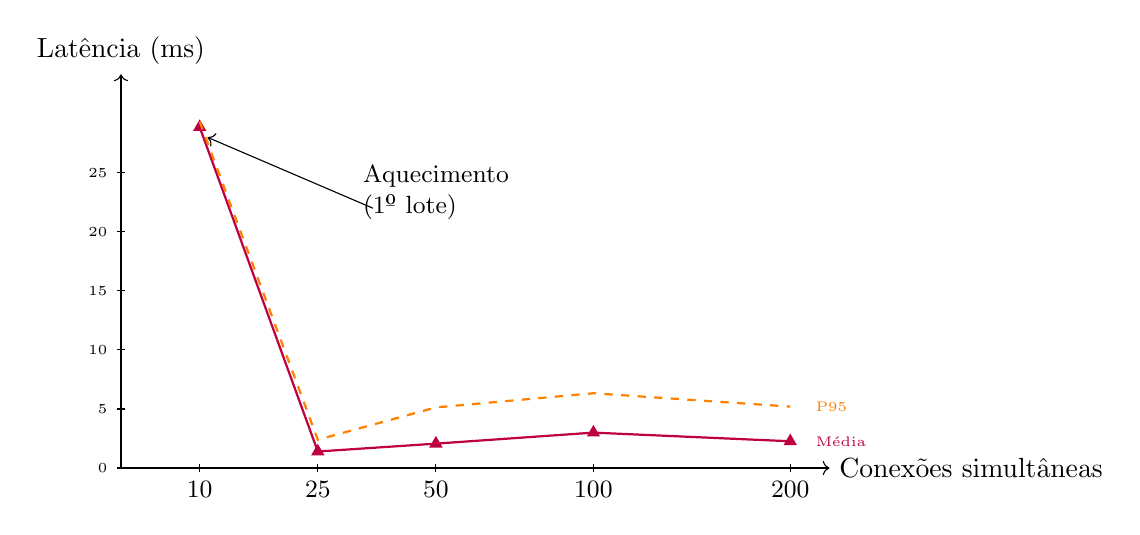
\begin{tikzpicture}
  % Axes
  \draw[->] (0,0) -- (9,0) node[right] {Conexões simultâneas};
  \draw[->] (0,0) -- (0,5) node[above] {Latência (ms)};

  % x ticks: 10(1), 25(2.5), 50(4.0), 100(6), 200(8.5)
  \foreach \x/\lbl in {1/10, 2.5/25, 4.0/50, 6/100, 8.5/200}
    \draw (\x,0.05) -- (\x,-0.05) node[below] {\small\lbl};

  % y ticks (1ms = 0.15cm)
  \foreach \y/\lbl in {0/0, 0.75/5, 1.5/10, 2.25/15, 3.0/20, 3.75/25}
    \draw (0.05,\y) -- (-0.05,\y) node[left,font=\tiny] {\lbl};

  % Join mean ms × 0.15: 28.85→4.33, 1.37→0.21, 2.06→0.31, 3.01→0.45, 2.27→0.34
  \draw[purple, thick, mark=triangle*, mark options={fill=purple}]
    plot coordinates {(1, 4.33) (2.5, 0.21) (4.0, 0.31) (6, 0.45) (8.5, 0.34)};

  % Join P95 × 0.15: 29.35→4.40, 2.37→0.36, 5.16→0.77, 6.35→0.95, 5.2→0.78
  \draw[orange, dashed, thick]
    plot coordinates {(1, 4.40) (2.5, 0.36) (4.0, 0.77) (6, 0.95) (8.5, 0.78)};

  \node[purple, right] at (8.7, 0.34) {\tiny Média};
  \node[orange, right] at (8.7, 0.78) {\tiny P95};
  \node[font=\small, align=left] at (4, 3.5) {Aquecimento \\ (1º lote)};
  \draw[->, thin] (3.2, 3.3) -- (1.1, 4.2);
\end{tikzpicture}
\fonte{Elaborado pelo autor.}
\end{figure}

\subsection{Interpretação dos Resultados}

Os dados obtidos confirmam as propriedades fundamentais do modelo de execução da BEAM/Erlang aplicado ao ExoGame:

\begin{enumerate}
  \item \textbf{Estabilidade sob carga}: a latência P95 permaneceu abaixo de 16 ms para todos os níveis de concorrência HTTP, sem degradação progressiva, o que indica ausência de contenção de recursos;
  
  \item \textbf{Escalabilidade horizontal imediata do WebSocket}: 200 conexões simultâneas foram estabelecidas sem erros, com \textit{join} médio de 2,3 ms, demonstrando que o padrão de processo-por-conexão da BEAM é viável mesmo em hardware de desenvolvimento;
  
  \item \textbf{Throughput elevado com recursos mínimos}: 3.249 req/s com zero erros em 8 segundos sustentados, em ambiente com 1 CPU e 2 GB de RAM, excede amplamente os requisitos de uma partida padrão do ExoGame (máximo de $\sim$30 jogadores, $\sim$5 perguntas, $\sim$150 eventos WebSocket por partida);
  
  \item \textbf{Implicações para o Docker Compose}: o \textit{container} do \textit{backend} com limite de 1 CPU e 1 GB de RAM (definido no \texttt{docker-compose.yml}) atende confortavelmente cargas de dezenas de salas simultâneas, com margem para centenas de jogadores concorrentes sem necessidade de escalonamento horizontal.
\end{enumerate}

\section{Discussão}

A arquitetura adotada demonstrou-se adequada para os requisitos do sistema. A implementação utiliza exclusivamente \textbf{Phoenix 1.7 (Elixir/BEAM)} como \textit{backend}, escolha fundamentada nos resultados empíricos apresentados neste capítulo (\autoref{sec:desempenho}) e em casos consagrados de produção como o WhatsApp (\autoref{sec:whatsapp}), bem como na trajetória histórica do Elixir e do Erlang/OTP (\autoref{sec:historia_elixir}). O Phoenix sustentou \textbf{200 conexões WebSocket simultâneas sem erros}, com latência \textbf{estável e previsível} independentemente do nível de concorrência --- propriedades essenciais para garantir experiência uniforme a todos os jogadores de uma sala. A comunicação via Phoenix Channels (WebSocket nativo RFC~6455) proporcionou sincronização em tempo real com latência imperceptível, essencial para a experiência de quiz.

O armazenamento em memória via \texttt{GenServer} no Phoenix é adequado para o contexto acadêmico. Para persistência, a integração com Ecto/PostgreSQL seria o caminho natural para uma evolução da plataforma.

A Context API do React, utilizada para gerenciamento de estado no \textit{frontend}, mostrou-se suficiente para a complexidade atual da aplicação, evitando a sobrecarga de bibliotecas externas como Redux ou Zustand.


% ============================================================
% CAPÍTULO 7 - TRABALHOS FUTUROS
% ============================================================
\chapter{Trabalhos Futuros}\label{cap:trabalhos_futuros}

Este capítulo propõe extensões e melhorias para a plataforma ExoGame, com fundamentação teórica e técnica para cada proposta.

\section{Visualização 3D de Exoplanetas com Three.js}

Uma das extensões mais promissoras para a plataforma é a incorporação de \textbf{visualizações tridimensionais interativas} de exoplanetas utilizando a biblioteca \textbf{Three.js} \cite{threejs2024}. A proposta consiste em:

\begin{enumerate}
  \item \textbf{Integração com dados da NASA}: utilizar a API pública do NASA Exoplanet Archive \cite{nasaexoplanet2024} para obter parâmetros reais de exoplanetas confirmados, como raio, período orbital, distância da estrela hospedeira e temperatura estimada;
  
  \item \textbf{Renderização interativa}: criar cenas 3D que representem exoplanetas e seus sistemas estelares, com texturas procedurais geradas a partir de parâmetros físicos reais. O usuário poderia manipular a câmera, aplicar zoom e observar animações orbitais;
  
  \item \textbf{Contextualização no quiz}: após cada pergunta sobre um exoplaneta específico, exibir sua representação 3D como \textit{feedback} educativo, conectando o conhecimento abstrato a uma representação visual concreta;
  
  \item \textbf{Comparação visual}: permitir a sobreposição de exoplanetas com planetas conhecidos do Sistema Solar, facilitando a compreensão de escalas e proporções.
\end{enumerate}

A integração com Three.js no ecossistema React/Next.js pode ser facilitada pela biblioteca \texttt{@react-three/fiber}, que oferece uma interface declarativa para criação de cenas 3D. Essa extensão alinha-se com os princípios de visualização interativa de dados para educação \cite{murray2013}.

\section{Algoritmos de Recomendação para Trilhas de Aprendizagem}

A segunda proposta de extensão envolve a implementação de um \textbf{sistema de recomendação} capaz de personalizar a experiência de aprendizagem de cada jogador. O sistema funcionaria conforme descrito a seguir:

\subsection{Modelo de Desempenho do Aluno}

Para cada jogador, o sistema manteria um \textbf{perfil de aprendizagem} baseado em:

\begin{itemize}
  \item Taxa de acerto por categoria de questão (tipos de exoplanetas, métodos de detecção, zona habitável, etc.);
  \item Tempo médio de resposta por categoria;
  \item Evolução temporal do desempenho;
  \item Padrões de erro recorrentes.
\end{itemize}

\subsection{Algoritmo de Recomendação}

Com base no perfil do aluno, o sistema utilizaria técnicas de \textbf{filtragem baseada em conteúdo} \cite{ricci2011} para:

\begin{enumerate}
  \item \textbf{Adaptar a dificuldade}: selecionar questões com nível de dificuldade adequado à zona de desenvolvimento proximal do aluno \cite{vygotsky1978};
  \item \textbf{Priorizar lacunas}: apresentar mais questões sobre categorias com baixa taxa de acerto;
  \item \textbf{Reforçar acertos}: intercalar questões de categorias dominadas para manter a motivação e o senso de competência;
  \item \textbf{Sugerir materiais complementares}: recomendar artigos, vídeos e simulações com base nas áreas identificadas como deficitárias.
\end{enumerate}

Essa abordagem está fundamentada em pesquisas sobre aprendizagem adaptativa \cite{brusilovsky2007, klašnja2011}, que demonstram que sistemas personalizados produzem melhores resultados de aprendizagem em comparação com abordagens genéricas.

\section{Outras Melhorias Propostas}

Adicionalmente, propõem-se as seguintes melhorias:

\begin{itemize}
  \item \textbf{Persistência de dados}: migração do armazenamento em memória para banco de dados (MongoDB ou PostgreSQL) com cache Redis;
  \item \textbf{Autenticação}: implementação de sistema de login com JWT (\textit{JSON Web Token}) para rastreamento longitudinal do desempenho;
  \item \textbf{PWA (\textit{Progressive Web App})}: conversão para aplicação \textit{web} progressiva com suporte \textit{offline} e instalabilidade \cite{majchrzak2018};
  \item \textbf{Internacionalização}: suporte a múltiplos idiomas (português, inglês, espanhol);
  \item \textbf{Modo professor}: painel administrativo para criação e curadoria de questões, com métricas de desempenho da turma;
  \item \textbf{Acessibilidade}: implementação de suporte a leitores de tela, navegação por teclado e alto contraste.
\end{itemize}


% ============================================================
% CAPÍTULO 8 - CONCLUSÃO
% ============================================================
\chapter{Conclusão}\label{cap:conclusao}

Este trabalho apresentou o desenvolvimento da plataforma ExoGame, um sistema \textit{web} gamificado de perguntas e respostas em tempo real, projetado para a divulgação de conceitos astronômicos sobre exoplanetas. A plataforma foi construída com uma arquitetura cliente-servidor moderna, empregando Next.js 15 no \textit{frontend} e Phoenix 1.7 (Elixir) no \textit{backend}, com comunicação bidirecional em tempo real via Phoenix Channels (WebSocket nativo).

Os objetivos propostos foram atingidos de forma satisfatória:

\begin{enumerate}
  \item A \textbf{revisão bibliográfica} fundamentou teoricamente a plataforma nos campos de gamificação \cite{kapp2012, deterding2011, hamari2014}, tecnologias \textit{web} em tempo real \cite{lubbers2010, puranik2024} e ensino de Astronomia \cite{langhi2009};
  
  \item A \textbf{arquitetura técnica} foi projetada e implementada com sucesso, demonstrando a viabilidade da combinação Next.js + Phoenix/Elixir + Channels para aplicações educacionais interativas;
  
  \item As \textbf{mecânicas de gamificação} implementadas --- pontuação baseada em tempo, avatares, \textit{leaderboard} dinâmico e sistema de salas --- alinham-se com os fundamentos teóricos da Teoria da Autodeterminação \cite{ryan2000} e da Teoria do Fluxo \cite{csikszentmihalyi1990};
  
  \item A \textbf{documentação técnica} completa foi produzida, incluindo diagramas de arquitetura, tabelas comparativas e trechos de código comentados;
  
  \item As \textbf{propostas de trabalhos futuros} --- visualização 3D com Three.js e algoritmos de recomendação --- foram elaboradas com fundamentação teórica e viabilidade técnica.
\end{enumerate}

A principal contribuição deste trabalho reside na demonstração de que a integração de gamificação com tecnologias \textit{web} modernas constitui uma abordagem promissora e tecnicamente viável para engajar estudantes no aprendizado de conceitos astronômicos complexos. A plataforma ExoGame serve tanto como ferramenta educacional quanto como referência técnica para o desenvolvimento de aplicações semelhantes em outras áreas do conhecimento.

Como limitações, destaca-se a ausência de uma avaliação empírica formal com estudantes, o armazenamento exclusivamente em memória e a necessidade de curar um banco de questões específico sobre exoplanetas. Estas limitações, contudo, são endereçadas nas propostas de trabalhos futuros, que expandem significativamente o potencial da plataforma.

A astronomia, em sua essência, nos convida a olhar além do que é imediato e familar. Do mesmo modo, a tecnologia educacional nos desafia a ir além dos métodos tradicionais de ensino. A plataforma ExoGame representa um passo nessa direção: a união entre a curiosidade pelos mundos distantes e as possibilidades oferecidas pelas tecnologias \textit{web} contemporâneas.


% ----------------------------------------------------------
% ELEMENTOS PÓS-TEXTUAIS
% ----------------------------------------------------------
\postextual

% ----------------------------------------------------------
% Referências bibliográficas
% ----------------------------------------------------------
\bibliography{exogame-references}

% ----------------------------------------------------------
% Apêndices
% ----------------------------------------------------------
\begin{apendicesenv}

\partapendices

% ----------------------------------------------------------
\chapter{Estrutura de Diretórios do Projeto}\label{ap:estrutura}
% ----------------------------------------------------------

A seguir é apresentada a estrutura completa de diretórios do projeto ExoGame. O \textit{backend} --- único --- é \texttt{backend\_elixir/} (Phoenix/Elixir); o \textit{frontend} é \texttt{frontend/} (Next.js).

\begin{lstlisting}[language={}, caption={Estrutura de diretórios do projeto ExoGame}, label={lst:diretorios}]
exogame/
|-- package.json          # Scripts raiz
|-- start.sh              # Script de inicialização (Elixir + Next.js)
|-- docker-compose.yml    # Orquestração Docker (Phoenix + Next.js)
|-- backend_elixir/       # Backend - Phoenix/Elixir (BEAM)
|   |-- mix.exs                    # Dependências e configuração
|   |-- mix.lock                   # Lock de versões
|   |-- Dockerfile                 # Imagem Docker (produção)
|   |-- config/
|   |   |-- config.exs             # Configuração base
|   |   |-- dev.exs                # Configuração de desenvolvimento
|   |   |-- runtime.exs            # Configuração em tempo de execução
|   |-- lib/
|       |-- backend_elixir/
|       |   |-- application.ex    # Supervisão OTP (raiz)
|       |   |-- game_server.ex    # GenServer: lógica do jogo
|       |   |-- question_service.ex # Serviço de questões
|       |   |-- player_service.ex   # Serviço de jogadores
|       |-- backend_elixir_web/
|           |-- endpoint.ex        # Endpoint HTTP/WebSocket
|           |-- router.ex          # Roteamento HTTP REST
|           |-- channels/
|               |-- game_channel.ex # Canal WebSocket principal
|-- frontend/
    |-- next.config.ts
    |-- package.json
    |-- tsconfig.json
    |-- postcss.config.mjs
    |-- public/
    |-- src/
        |-- app/
        |   |-- globals.css
        |   |-- layout.tsx         # Layout raiz + GameProvider
        |   |-- page.tsx           # Roteamento por estado
        |-- components/
        |   |-- AvatarSelector.tsx
        |   |-- HomePage.tsx
        |   |-- Leaderboard.tsx
        |   |-- Lobby.tsx
        |   |-- PlayerHeader.tsx
        |   |-- QuestionView.tsx
        |-- contexts/
        |   |-- GameContext.tsx     # Estado global + Phoenix Channels
        |-- types/
            |-- game.types.ts      # Interfaces frontend
\end{lstlisting}

% ----------------------------------------------------------
\chapter{Diagrama de Fluxo da Partida}\label{ap:fluxo}
% ----------------------------------------------------------

A \autoref{fig:fluxo_partida} apresenta o diagrama de fluxo completo de uma partida no ExoGame.

\begin{figure}[htb]
\caption{\label{fig:fluxo_partida}Diagrama de fluxo de uma partida no ExoGame}
\begin{center}
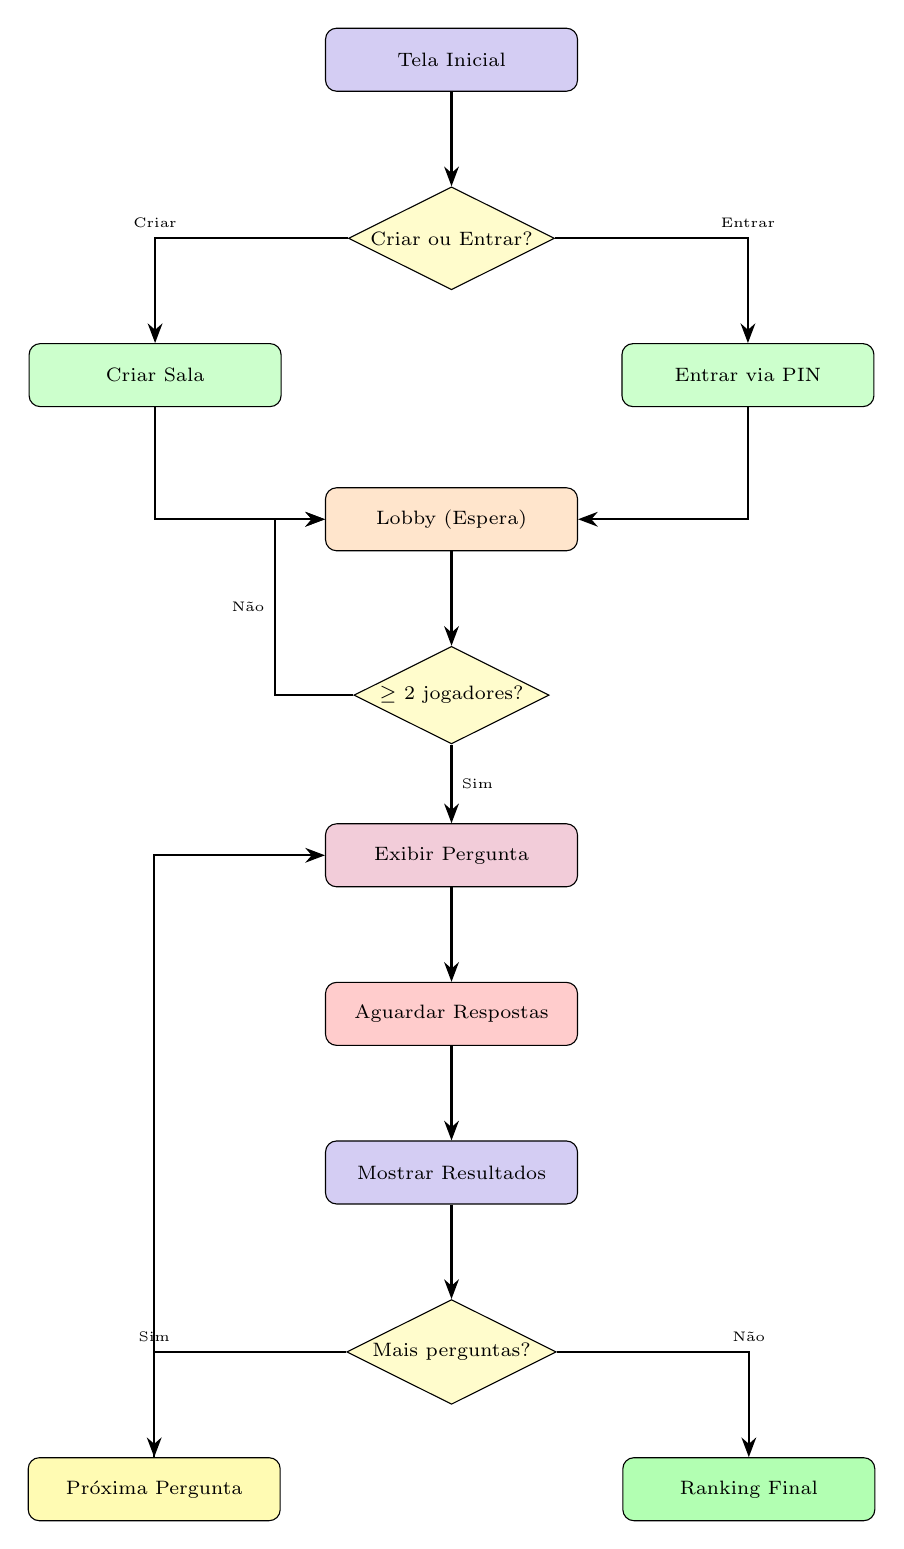
\begin{tikzpicture}[
  node distance=1.2cm,
  state/.style={rectangle, draw, rounded corners, minimum width=3.2cm, minimum height=0.8cm, text centered, font=\scriptsize, fill=#1},
  decision/.style={diamond, draw, aspect=2, minimum width=2cm, text centered, font=\scriptsize, fill=yellow!20, inner sep=1pt},
  arrow/.style={-{Stealth[length=2.5mm]}, thick},
]

\node[state=blue!20] (inicio) {Tela Inicial};
\node[decision, below=of inicio] (opcao) {Criar ou Entrar?};
\node[state=green!20, below left=1cm and 1.5cm of opcao] (criar) {Criar Sala};
\node[state=green!20, below right=1cm and 1.5cm of opcao] (entrar) {Entrar via PIN};
\node[state=orange!20, below=2.5cm of opcao] (lobby) {Lobby (Espera)};
\node[decision, below=of lobby] (minimo) {$\geq$ 2 jogadores?};
\node[state=purple!20, below=1cm of minimo] (pergunta) {Exibir Pergunta};
\node[state=red!20, below=of pergunta] (responder) {Aguardar Respostas};
\node[state=blue!20, below=of responder] (resultado) {Mostrar Resultados};
\node[decision, below=of resultado] (mais) {Mais perguntas?};
\node[state=yellow!30, below left=1cm and 1.5cm of mais] (proximo) {Próxima Pergunta};
\node[state=green!30, below right=1cm and 1.5cm of mais] (fim) {Ranking Final};

\draw[arrow] (inicio) -- (opcao);
\draw[arrow] (opcao) -| node[above, font=\tiny] {Criar} (criar);
\draw[arrow] (opcao) -| node[above, font=\tiny] {Entrar} (entrar);
\draw[arrow] (criar) |- (lobby);
\draw[arrow] (entrar) |- (lobby);
\draw[arrow] (lobby) -- (minimo);
\draw[arrow] (minimo) -- node[right, font=\tiny] {Sim} (pergunta);
\draw[arrow] (minimo.west) -- +(-1,0) |- node[left, font=\tiny, pos=0.25] {Não} (lobby.west);
\draw[arrow] (pergunta) -- (responder);
\draw[arrow] (responder) -- (resultado);
\draw[arrow] (resultado) -- (mais);
\draw[arrow] (mais) -| node[above, font=\tiny] {Sim} (proximo);
\draw[arrow] (proximo) |- (pergunta);
\draw[arrow] (mais) -| node[above, font=\tiny] {Não} (fim);

\end{tikzpicture}
\end{center}
\legend{Fonte: Elaborado pelo autor.}
\end{figure}

% ─── Apêndice C – Docker Compose ──────────────────────────────────────────
\chapter{Configuração Docker Compose}

O arquivo \texttt{docker-compose.yml} abaixo define a configuração completa para implantar a plataforma ExoGame em contêineres Docker, com restrições de recursos adequadas a um servidor de demonstração ou ambiente de avaliação acadêmica. O \textit{backend} é o \textbf{Phoenix/Elixir (BEAM)} --- escolhido por sua reconhecida superioridade em aplicações WebSocket de alta concorrência, conforme discutido na \autoref{sec:whatsapp} --- e o \textit{frontend} é o Next.js com saída \textit{standalone}.

\begin{lstlisting}[caption={docker-compose.yml -- orquestração dos serviços ExoGame (backend Phoenix/Elixir)},
                   label={lst:docker_compose}]
services:
  # Backend - Phoenix / Elixir (BEAM)
  backend:
    build:
      context: ./backend_elixir
      dockerfile: Dockerfile
    container_name: exogame_backend
    restart: unless-stopped
    environment:
      MIX_ENV: production
      PHX_SERVER: "true"
      PORT: "3001"
      PHX_HOST: "localhost"
      SECRET_KEY_BASE: "<gere com: mix phx.gen.secret>"
    ports:
      - "3001:3001"
    networks:
      - exogame_net
    deploy:
      resources:
        limits:
          cpus: "1.0"
          memory: 1024M
        reservations:
          cpus: "0.25"
          memory: 256M
    healthcheck:
      test: ["CMD","wget","--quiet","--tries=1","--spider",
             "http://localhost:3001/questions"]
      interval: 15s
      timeout: 5s
      retries: 5
      start_period: 30s

  # Frontend - Next.js (standalone)
  frontend:
    build:
      context: ./frontend
      dockerfile: Dockerfile
    container_name: exogame_frontend
    restart: unless-stopped
    environment:
      NODE_ENV: production
      NEXT_PUBLIC_BACKEND_URL: "http://localhost:3001"
      NEXT_PUBLIC_BACKEND_WS:  "ws://localhost:3001"
    ports:
      - "3000:3000"
    networks:
      - exogame_net
    depends_on:
      backend:
        condition: service_healthy
    deploy:
      resources:
        limits:
          cpus: "1.0"
          memory: 1024M
        reservations:
          cpus: "0.25"
          memory: 256M
    healthcheck:
      test: ["CMD","wget","--quiet","--tries=1","--spider",
             "http://localhost:3000"]
      interval: 15s
      timeout: 5s
      retries: 5
      start_period: 60s

networks:
  exogame_net:
    driver: bridge
\end{lstlisting}

Para iniciar a aplicação completa em ambiente Docker, basta executar:

\begin{lstlisting}[language={}]
docker compose up --build
\end{lstlisting}

O \textit{backend} estará disponível em \texttt{http://localhost:3001} e o \textit{frontend} em \texttt{http://localhost:3000}. O Compose aguarda a verificação de saúde (\textit{healthcheck}) do \textit{backend} antes de iniciar o \textit{frontend}, garantindo que a dependência de serviços seja respeitada.

\end{apendicesenv}

% ----------------------------------------------------------
% Índice remissivo
% ----------------------------------------------------------
\phantompart
\printindex

\end{document}
